\documentclass[subeqn]{article}

\title{The Twin Instrument\footnote{We are grateful to Paul Devereux, James 
Fenske, Cheti Nicoletti, Carol Propper, Atheen Venkataramani, Marcos 
Vera-Hernandez and Frank Windmeijer, along with various seminar audiences and 
discussants for helpful comments.  We thank Emilia Del Bono, Climent 
Quintana-Domeque, Pedro R\'odenas, Libertad Gonz\'alez, Hanna M\"uhlrad, Anna 
Aevarsdottir, Martin Foureaux Koppensteiner and Ryan Palmer who have very 
kindly shared data and/or source code from their work.}}
\author{Sonia Bhalotra\thanks{The University of Essex.
Contact: \href{mailto:srbhal@essex.ac.uk}{srbhal@essex.ac.uk}} 
\and Damian Clarke\thanks{The University of Oxford. 
Contact: \href{mailto:damian.clarke@economics.ox.ac.uk}
{damian.clarke@economics.ox.ac.uk}}}
\date{August 2015}

%at CMPO Bristol, ESPE, NEUDC, CSAE, The University of Essex, The University of 
%Oxford, the Barcelona GSE summer forum, PacDev, and the RES conference

%*******************************************************************************
\usepackage{amsmath}
\usepackage{amssymb}
\usepackage{appendix}
\usepackage{blindtext}
\usepackage{bm}
\usepackage{booktabs}
\usepackage{breqn}
\usepackage{caption}
\usepackage[usenames, dvipsnames]{color} \pagecolor{white}
\usepackage{dcolumn}
\usepackage{epsfig}
\usepackage{epstopdf}
\usepackage[capposition=top]{floatrow}
\usepackage{hyperref}
\usepackage{lastpage}
\usepackage{longtable}
\usepackage{lscape}
\usepackage{multirow}
\usepackage{natbib} \bibliographystyle{abbrvnat}\bibpunct{(}{)}{;}{a}{,}{,}
\usepackage{pdfpages}
\usepackage{rotating}
\usepackage{setspace}
\usepackage{subcaption}
\usepackage{subfloat}
\usepackage{url}
\usepackage{wrapfig}


%*******************************************************************************
\setlength\topmargin{-0.375in}
\setlength\textheight{8.8in}
\setlength\textwidth{5.8in}
\setlength\oddsidemargin{0.4in}
\setlength\evensidemargin{-0.5in}
\setlength\parindent{0.25in}
\setlength\parskip{0.25in}

\hypersetup{                                                                                                    
    colorlinks=true,   
    linkcolor=BlueViolet,
    citecolor=BlueViolet,
    filecolor=BlueViolet,
    urlcolor=BlueViolet
}


\newcommand{\twinfolder}{"/home/damiancclarke/investigacion/Activa/Twins"}
\DeclareMathOperator{\plim}{plim}

%*******************************************************************************
\begin{document}
\begin{spacing}{1.4}

\maketitle
\vspace{-1cm}
%\begin{center}{\Large\textsc{Preliminary Draft}}\end{center}
\begin{abstract}
 The incidence of twins has been used to identify the impact of changes in 
 fertility on measures of investment in children born prior to the twins, and
 the emerging consensus in this literature is that there is no evidence of a
 quantity-quality (Q--Q) trade-off. We argue that the standard approach is 
 flawed. Even if twin conception is random, bringing twins to term is a function 
 of maternal health which is difficult to fully observe and which tends to be
 correlated with child quality, rendering the instrument invalid. The neglect
 of this fact in the existing literature will tend to lead to under-estimation 
 of the Q--Q trade-off and so could contribute to explaining the negative results
 in the literature. Our contention that women who produce twin births are
 positively selected is demonstrated using data from richer and poorer countries.
 Using large samples of microdata from developing countries and from the USA 
 which include indicators of maternal characteristics including health, we show
 that a significant trade-off emerges upon correcting for these biases. We show
 that this result is likely to be only a \emph{lower} bound of the true Q--Q
 trade-off and discuss how to estimate the size of these bounds. These results
 have important implications for twin studies in all contexts examined here.
\\
\end{abstract}
\hspace{4mm}\textbf{\small JEL codes}: J12,J13,C13,D13,I12. \\

\newpage
%*******************************************************************************
\section{Introduction}                             \label{TWINscn:intro}
Since the pioneering work of \citet{RosenzweigWolpin1980}, economists have 
attempted to leverage the occurrence of twin births to estimate the effect of 
family size on child outcomes. If twin births occur at random, their occurrence 
constitutes a fertility shock that is uncorrelated with family characteristics, 
including parental preferences, and other unobservables which may be related to 
child quality. This provides the exogenous variation (in quantity) required to 
estimate the quantity-quality model of \citet{Becker1960,BeckerLewis1973,
BeckerTomes1976}.  The essential idea of these studies is that the shadow price 
of child quality is increasing in child quality and \emph{vice versa}.  By 
comparing those families who unexpectedly produced additional children with 
those who always produced one child per birth, it is argued that the effect of 
an additional sibling on a child's human capital attainment can be identified.

However, the consistent estimation of this effect is based upon the untestable 
assumption that twinning is exogenous. This requires not only that twin 
conceptions are randomly assigned to families, but also that taking a twin
conception to term does not depend upon a woman's behaviours during pregnancy 
or on her endowments prior to pregnancy. This is at odds with the evidence.

We show that endowments and behaviours affect the chances of twins being born. 
In data from a large sample of developing countries, we show that taller women 
and women with a higher body-mass index are significantly more likely to give 
birth to twins.\footnote{Height is an index of the stock of health of a woman 
and is a function of investments over her growth period and, especially, the 
early years of her life (see references in \citet{BhalotraRawlings2013}).} 
Maternal health is likely to be an especially significant determinant of birth 
outcomes in poorer countries where many women are chronically under-nourished 
(an indicator of which is their final stature), exhibit anemia and low-BMI, and 
are prone to infections. In these conditions only relatively healthy women will 
have the resources to support a successful twin pregnancy. However, our critique 
applies to richer countries too. Using administrative data from the Scotland,
the USA, Sweden and Spain, and survey data from the UK and Chile, we find that 
women who are taller and less likely to engage in risky behaviours such as 
smoking, drug taking or alcohol consumption during pregnancy are significantly 
more likely to have a (live) twin birth.\footnote{Simiarly, it is well known 
that fertility treatments increase the likelihood of twinning. While we do not 
discuss this extensively here, we note that this is likely to be less of an 
identification challenge given that IVF treatment is an entirely observable 
behaviour.}

Overall, our argument is that women who give birth to twins are positively 
selected and that the common tendency to ignore this will result in under-%
estimation of the Q--Q trade-off. We focus upon maternal health because no 
previous work has highlighted it as a determinant of twinning, and because it is 
inherently impossible to fully control for. Even if we had data that included 
all of the indicators of health we mention above, we may not observe whether 
women skip breakfast \citep{MazumderSeeskin2014}, whether they are stressed 
(\citet{Blacketal2014} and references therein), whether they seek and adhere to 
antenatal care and so on. Our contention adds a novel twist to a recent 
literature which suggests that mothers' health and fetal environment matter and 
may alter the birth weight of children, the sex ratio at birth and a range of 
future human capital outcomes \citep{Almondetal2011,BhalotraRawlings2013,
Barker1995}. Like birth weight and the probability of a boy relative to a girl 
birth, the probability of a twin birth is increasing in the health of the 
mother/the fetal environment.

The emerging consensus in the literature using twin births to test the Q--Q 
model is that there is in fact no significant or substantial trade-off between 
fertility and investments in children. In this paper we suggest that this result 
may, in principle, follow from the bias created by twin-mothers being positively 
selected. We re-examine the validity of these results, accounting for the 
innovation discussed previously.  If twin births are not truly exogenous, but 
instead depend upon maternal health stocks and behaviours, there is an 
identification challenge.  Specifically, if healthier mothers are both more 
likely to give birth to twins, and more likely to invest in child human capital 
in later life, existing estimates may significantly underestimate the size of the 
Q--Q trade-off.  When ignoring these considerations we find that the effect of an 
additional birth on human capital attainment (education) is minor, or even weakly 
positive. However, when taking into account this innovation we find that a 
significant trade-off does exist, and that an additional birth reduces 
standardised schooling behaviour by at least 4\% of a standard deviation.

The estimated effect of $\sim 4\%$ of an s.d.\ is at most the lower bound for 
the true size of the Q--Q trade-off. Given that we suggest that maternal health 
predicts twinning, and given that maternal health is multidimensional in nature 
and difficult to observe fully, we will only ever be able to include a partial 
set of controls to account for the inconsistency in IV estimates. As such, we 
examine a number of methods to estimate plausible bounds on the Q--Q trade-off. 
First, we argue that the true estimate is bounded by the OLS and IV estimtes. 
We also follow \citet{Conleyetal2012} in conceptualizing twins as a plausibly 
exogenous event, and derive estimates by assuming that the traditional exclusion 
restriction is `close to' holding.

Empirically, work which further probes the Q--Q trade-off is important,
especially in the developing country setting on which we place considerable 
focus in this paper. In order to conduct empirical tests, we construct a large 
microdata set from 68 developing countries with observations on more than 2.5 
million children and nearly 1 million mothers. The macro level trends in this 
data suggest that educational attainment has risen considerably while completed 
and desired fertility has fallen sharply over the past 50 years (see figures 
\ref{TWINfig:fertrend} and \ref{TWINfig:eductrend}). Similar effects have been 
described extensively in the economic and demographic literature (\emph{eg} 
\citet{Hanushek1992}). It is of considerable relevance to researchers and to 
policy makers to determine whether such a trend is (at least partially) causal.
In practical terms, a significant number of government bodies report that
family planning is considered an important concern,\footnote{A recent survey of 
national governments suggests that fertility was perceived as too high in 50\% 
of developing countries, with this figure rising to 86\% among the least 
developed countries \citet{UN2010}.}  and in some cases these concerns have 
resulted in aggressive, and at times group-specific, fertility control 
policies.  %We then examine the Q--Q trade-off using a decade's worth of 
%representative survey data from the United States.  In this context both 
%desired and completed fertility are lower, 

This paper unfolds as follows. In the next section we discuss the existing 
literature which estimates the Q--Q model using twins. We then discuss the 
methodology that we will use to examine twinning, and to bound the Q--Q 
trade-off.  Section \ref{TWINscn:data} discusses our data sources and estimation 
samples, and section \ref{TWINscn:results} presents results. We briefly conclude 
in the final section.

%*******************************************************************************
\section{Twins}                                    \label{TWINscn:literature}
The ocurrence of twins has fascinated people, not least of all social 
scientists, for as long as recorded history exists. Stories of Romulus and 
Remus, the mythological founders of Rome, date from at least the fourth century 
BC. However, the first use of twins as an exogenous increase in family size in 
the economic literature came much later, in \citet{RosenzweigWolpin1980}.

\citet{RosenzweigWolpin1980} proposed to incorporate twins into an estimation
strategy in order to circumnavigate problems of the joint determination of child 
quantity and quality first raised by \citet{Becker1960,BeckerLewis1973,
BeckerTomes1976}.  Under a number of assumptions, they show that twins as an 
increase to family size will be sufficient to directly identify the interaction
between quality and quantity.  As well as the occurrence of twins pushing at
least some families above their desired total fertility, this requires that 
twin births are random.  Empirically then, \citet{RosenzweigWolpin1980} estimate 
the Q--Q trade-off, accounting for the increase in rates of twinning by parity 
(a biological relationship)\footnote{Such a relationship is an empirical 
regularity in all data examined. \citet{RosenzweigWolpin1980} report rates which 
increase by parity in USA.  In DHS data a similar pattern is observed, as 
presented in figure \ref{TWINfig:bord}.}, and by total number of births (a 
mechanical relationship).  Beyond these variables, twinning must be random to
produce consistent estimates.\footnote{It is important to note that in their
original paper this \emph{is} tested formally.  The authors report that a joint
test of the effect of farm size, non-farm earnings and parental education on the
rate of twins per births did \emph{not} allow for the rejection of no 
statistical effect.}

The twin instrument has been widely used since \citeauthor{RosenzweigWolpin1980}'s
(\citeyear{RosenzweigWolpin1980}) initial work. As well as its use in the 
estimation of the quantity-quality trade-off (\citet{Blacketal2005,Caceres2006,
Lietal2008,Angristetal2010}, among others), it has been used to 
estimate the effect of childbearing on female labour force participation 
\citep{RosenzweigWolpin1980b,Jacobsenetal1999,AngristEvans1998}, and the effect 
of unwed childbearing on marriage market outcomes, poverty and welfare receipt 
\citep{BronarsGrogger1994}.  Typically, estimation is based on two-stage least
squares, with the set of controls included in the first- and second-stage 
varying slightly over time.\footnote{Twins have been widely used in the economic, 
medical, biology and psychology literature in a number of ways.  In this paper 
we focus only on the use of twin births as an instrument for total fertility, 
and not on the so called `twin studies', which base inference on between-twin 
comparisons using maternal fixed effects.}

Table \ref{TWINtab:Lit} documents the principal studies in the Q--Q trade-off 
literature where twins are employed.  Along with the data sample and time period 
under study, we list the set of controls included in each case.  The more recent
wave of these studies make a similar conditional randomness assumption, however
refurbish the controls in IV estimates to include variables such as a mother's 
race and her educational attainment.  In some cases the validity of such 
assumptions is probed by regressing twinning on observable family outcomes, or 
testing for the equality of means of certain characteristics between twin and
non-twin families. \citet{Blacketal2005}, \citet{Lietal2008} and 
\citet{Sanhueza2009} report joint F-tests suggesting that twinning is not related 
to parental education in their data samples, while \citet{RosenzweigZhang2009} 
report t-tests showing equality of means across twin and non-twin groups. 
However, as is well known and acknowledged in each case, any such tests are at 
best partial evidence in support of instrumental validity. While twins can be 
shown to be unrelated to observable or measured characteristics, similar tests 
cannot be run for variables which are either unobservable, or not recorded in 
survey data. We return to this point in the following sections.

The most comprehensive controls considered in the economic literature (often by
necessity due to data restrictions), include maternal age, parental education
and measures of income and/or goods.  However, recent evidence from the medical
literature points to the fact that twinning may depend more deeply upon a 
mother's health behaviours or endowments. \citet{Hall2003} for example suggests 
that follicle-stimulating hormone (FSH) is associated with an increased 
likelihood of twinning, and is found in higher concentrations in older, heavier 
and taller mothers. Further, she suggests ``that adequate maternal folic acid 
consumption could affect the number of twins coming to term'' (see p.\ 741, and 
further discussion in \citet{Lietal2003}).

Unrelated to health measures \emph{per se}, recent studies seek to control for 
the fact that multiple births are correlated with fertility treatments. 
Typically, such an analysis requires either focusing on offspring born before
the introduction of fertility treatments \citep{Caceres2006,Angristetal2010}, 
or, in the case of sufficiently rich data, removing families undergoing fertility 
treatment from estimation samples \citep{Braakman2014}. Once again, consistent 
estimation in this case is based on the assumption that beyond fertility 
treatment and family controls listed above, twin births are as good as random.

Finally, the twin instrument is not without critique for other reasons. Existing
critiques of the twin instrument have focused on parental behaviours in response 
to twins, rather than on the likelihood that parental behaviours (or endowments) 
may affect the likelihood of twinning. \citet{RosenzweigZhang2009} question the 
effect that close (or indeed no) birth spacing and an endowment effect---where 
parental behaviours respond to the lower health at birth of twins compared to 
single births\footnote{Using data from the United States, \citet{Almondetal2005} 
document that twins have substantially lower birth weight, lower APGAR scores, 
higher use of assisted ventilation at birth and lower gestion period than 
singletons. In our data samples similar endowment differences are observed. For
example, appendix figure \ref{TWINfig:Size} documents the much larger average 
reported birth size of twins versus singletons in DHS data. Birth weight figures 
show similar patterns.}---has on investments in pre-twin siblings. They 
demonstrate that if parents behave in such a manner, bounds for the Q--Q 
trade-off can be calculated. This hypothesis is tested in 
\citet{Angristetal2010}, and applied in \citet{FitzsimonsMalde2014}.  We turn
to bounds estimation in section \ref{TWINsscn:resultBounds} of this paper.

%*******************************************************************************
\section{Methodology}                              \label{TWINscn:method}
Empirical analyses of the quality-quantity trade-off focus on producing 
consistent estimates of $\beta_1$ in the following equation:
\begin{equation}
\label{TWINeqn:RF}
educ_{ij}=\beta_0+\beta_1 fert_{j} + \bm{X}\bm{\beta}+u_{ij}.
\end{equation}
Here, quality is proxied by the educational attainment of child $i$ in family 
$j$, ($educ$) and fertility ($fert$) is measured as the total births in a child's
family.  A vector of family and child controls is included, denoted $\bm{X}$.  As
has been extensively discussed in prior literature, estimation of $\beta_1$ using
OLS with cross-sectional data will result in biased coefficients given that child 
quality and quantity are jointly determined \citep{BeckerLewis1973,
BeckerTomes1976}, and given that unobservable parental behaviours and attributes 
influence both fertility decisions, and investments in children's education 
\citep{Qian2009}.

%*******************************************************************************
\subsection{Quantity-Quality with Twins}           \label{TWINsscn:methodQQ}
One proposed solution has been to employ 2SLS estimation, where fertility is 
is instrumented using twin births.\footnote{Other instruments and methodologies 
are also used including gender mix of children \citep{ConleyGlauber2006}, policy 
experiments \citep{Qian2009}, and historical time series variation in schooling 
\citep{BleakleyLange2009}}  The corresponding first stage is:
\begin{equation}
\label{TWINeqn:firststage}
fert_{j}=\pi_0+\pi_1 twins_{j}+\bm{X}\bm{\pi}+\nu_{j},
\end{equation}
where $twins_j$ is an indicator for whether the $n^{th}$ birth in a family is a 
twin birth. As described further in section \ref{TWINsscn:samples}, the sample 
in each case is the so-called $n+$ group, consisting of children born before 
birth $n$ in families with at least $n$ births. As such the twins themselves are 
excluded from the estimation sample.\footnote{Typically, the argument is made 
that twins are different to single births, and hence should not be compared in 
analysis.} The logic, in quasi-experimental terms, is that existing children 
(the subjects) are randomly assigned either one (control group) or two 
(treatment group) siblings at the $n^{th}$ birth.

Consistent estimation of $\beta_1$ can thus proceed provided (among other
things) that instrumental validity holds:
\begin{equation}
\label{TWINeqn:IVvalid}
\plim_{N\to \infty} \frac{1}{N}\sum_{j=1}^N twin_ju_{ij}=0
\end{equation}
The typical challenge in IV estimates arises when considering 
(\ref{TWINeqn:IVvalid}); as the error term $u_{ij}$ consists, by nature, of 
unobservable components, whether or not the equality holds cannot be tested 
formally.  There is however nothing which stops us from partially testing 
(\ref{TWINeqn:IVvalid}) by removing a subset of observable components from $u_{ij}$
and testing whether their (conditional) correlation with $twin_j$ is 
significantly different from zero. The error term $u$ in (\ref{TWINeqn:RF}) 
is a function of a large number of elements:
\begin{equation}
\label{TWINeqn:IVbias}
\begin{split}
u=f(\text{maternal health stocks, fertility behaviour, positive pregnancy investments,}  \\
\text{parental education, fetal environment,}\ldots)
\end{split}
\end{equation}
While many of the relevant elements are either completely or partially 
unobservable, some of these variables, such as maternal education and 
incomplete measures of health stocks and behaviours, can be observed.  Thus a 
partial test of the twin methodology consists of estimating the following 
regression:
\begin{equation}
\label{TWINeqn:twinreg}
twin_{j}=\alpha_0 + \bm{X}\bm{\alpha}_1 + \bm{S}\bm{\alpha}_2
                  + \bm{H}\bm{\alpha}_3 + \varepsilon_{j}.
\end{equation}
Here $\bm{X}$ refers to the initial vector of family and child controls, $\bm{S}$
to additional family socioeconomic variables such as income and parental 
education, and $\bm{H}$ to maternal health variables.  

If twin birth is indeed an event which is as good as random, the coefficients
on maternal health and family socieoeconomic variables in the above regression
should not be significantly different to zero.  We thus test the following 
hypothesis:
\begin{equation}
\label{TWINeqn:twintest}
H_0: \bm{\alpha}_2 = \bm{\alpha}_3 = 0.
\end{equation}
Rejection of the null would raise difficulties in proceeding with IV estimation 
using the twin instrument. Of course, if the rejection of the null were only due 
to one or a number of \emph{observable} element(s) which predicted twinning, 
these variables could simply be included in the first and second stages above, 
much like occurs with maternal age and race in the existing literature.  However, 
more generally it would be difficult to be argue for instrumental validity if 
twinning is shown to depend upon (a limited set of) measurable family 
characteristic or choice variables, while many similar variables are not observed.

Given the biological demands placed on a mother pregnant with twins, we may 
expect that healthier mothers, or mothers with more resources to invest in their
pregnancy, are more likely to take twin conceptions to term.  Similarly, we may
suspect that mothers more able to invest in their children during pregnancy will 
also be more able to invest in their child's human capital after birth.  If this 
is the case, we would see that (at the very least) $\bm{\alpha}_2>0$.  

An alternative test of whether twins appear to be as good as random consists of 
comparing women who give birth to twins with those who give birth to singletons 
\emph{before} these children are born.  If twin births occur randomly in the 
population, the two groups of mothers should appear identical before these births 
occur. In order to compare health stocks before twins, we run tests comparing the 
rate of infant mortality---a completely predetermined variable---of children in 
each of the $n+$ groups described above.  If, as we contend, healthier mothers 
are more likely to give birth to twins, this should be captured in lower infant 
mortality rates (IMR) among twin mothers in early births.

If, following the tests described above, twins are found to be positively selected
among healthy mothers, traditional IV estimates of $\beta_1$ will be inconsistent.
We turn to discuss this bias now.
Assuming additive separability of the elements in the omitted error term\footnote{%
This assumption can be loosened with little implication on the analysis which
follows.  If we do not assume additive seperability, covariance terms between each
error component must be included.  However, given that the covariance between 
elements of $\bm{S}$ and $\bm{H}$ is likely to be positive, and given that the 
covariance between each of these and $u^*_{ij}$ is likely to be of the same sign
as the covariance between $twin$ and $u^*_{ij}$, the omission of the covariance
terms does not effect the inequalities in equation \ref{TWINeqn:moves}.  This is
something which we test empirically later in this paper.}, we can 
re-write $u_{ij}$ from (\ref{TWINeqn:firststage}) and (\ref{TWINeqn:IVbias}) as:
\[ u_{ij}=u^S_{ij}+u^H_{ij}+u^*_{ij}. \]
Here $u^S_{ij}$ and $u^H_{ij}$ correspond to the (observable) elements included 
as $\bm{S}$ and $\bm{H}$ in (\ref{TWINeqn:twinreg}), while $u^*_{ij}$ represents 
the remaining (unobserved) components.  We can thus re-write our IV estimate for 
$\beta_1$ as:
\begin{equation}
\label{TWINeqn:betabias}
\hat\beta_1^{IV} = \beta_1 + 
\plim_{N\to \infty} \frac{1}{N}\sum_{j=1}^N twin_j(u^S_{ij}+u^H_{ij}+u^*_{ij})
\end{equation}
Typically, this is the coefficient estimated in the existing twin literature 
which assumes that twinning is a conditionally exogenous event.  If, however, the 
likelihood of taking twin conceptions to term increases for healthier and/or 
wealthier mothers, we should include $\bm{S}$ and $\bm{H}$ in the first and 
second stages, giving
\begin{equation}
\label{TWINeqn:betacloser}
\hat\beta_1^{IV,S+H} = \beta_1 +
\plim_{N\to \infty} \frac{1}{N}\sum_{j=1}^N twin_ju^*_{ij},
\end{equation}
where the superscript $S+H$ signifies that socioeconomic and health variables 
have been included as additional controls and, correspondingly, have been 
removed from the stochastic error term.  What's more, if both the likelihood
that a woman takes twins to term, and a family's subsequent investment in child 
human capital, are positively correlated with positive health behaviours and other 
positive socioeconomic variables such as parental education, we would expect%
\footnote{This follows from the remainder terms in (\ref{TWINeqn:betabias}) and 
(\ref{TWINeqn:betacloser}).  If twinning is positively correlated with the
omitted error term in the second stage equation, any $\beta_1$ estimates will be
over-stated.} that:
\begin{equation}
\label{TWINeqn:moves}
\hat\beta_1^{IV}>\hat\beta_1^{IV,H}>\hat\beta_1^{IV,S+H}>\beta_1.
\end{equation}
It should be noted in the above series of inequalities that even conditional upon
socioeconomic and health variables, IV estimation will \emph{not} result in a
consistent estimate of $\beta_1$ if twinning is correlated with unobservable
elements in $u^*_{ij}$.  We return to this point, and how to bound $\beta_1$ in
the following sub-section.

%NOTE: Angrist Pischke first stage F-statistics when more than one endogenous
%regressor.
%*******************************************************************************
\subsection{Bounding the Q-Q Trade-off}            \label{TWINsscn:methodBounds}
In the previous subsection, Q-Q estimation using twins is motivated in equations 
(\ref{TWINeqn:RF}) and (\ref{TWINeqn:firststage}).  Consistent IV estimation 
imposes the (strong) prior belief that twin births can be excluded from the 
second stage equation, or that the sign of $\gamma$ in the following is equal to 
zero:
\begin{equation}
\label{TWINeqn:Conley}
educ_{ij}=\beta_1 fert_j + \gamma twin_j + \bm{X}\bm{\beta} + u_{ij}.
\end{equation}
As we discuss above, this will not be the case if maternal health controls 
omitted from (\ref{TWINeqn:RF}) are correlated with both the likelihood of 
taking twin conceptions to term, and with eventual measures of child quality.

However, even in cases such as this where we are not confident that $\gamma=0$,
we can still estimate bounds on the Q-Q tradeoff if we are confident in making
some statement of prior belief about the distribution from which $\gamma$ is 
drawn.  \citet{Conleyetal2012} describe such a process, which they refer to as 
\emph{plausible exogeneity}.\footnote{\citet{NevoRosen2012} propose a bounds
estimate for IV of a similar nature.  Inference in this case depends on 
assumptions about the direction of correlation between the instrument and the 
error term. They denote this as $\rho_{z_{j}u}$, which is analogous to the sign 
of $\gamma$ in \citeauthor{Conleyetal2012}'s framework which we apply here.} We 
invoke this terminology here, and refer to twins as a plausibly exogenous event, 
implying that we have reason to believe that $\gamma$ may be close to, but not 
necessarily precisely equal to, zero. Specifically, we are concerned that 
healthier mothers are more likely to give birth to twins, and, all else 
constant, healthier mothers are more likely to be able to invest more in their 
children post-pregnancy.  Thus, $\gamma$, the coefficient on twins in 
(\ref{TWINeqn:Conley}), reflects the interaction between the partial correlation 
of a mother's health and her likelihood of giving birth to twins, which we 
denote $\phi_t$, and the partial correlation between her health and child 
quality, denoted $\phi_q$.

In this paper we estimate $\beta_1$ under a range of assumptions regarding the
true nature of $\gamma$.  Firstly we estimate $\beta_1$ by simply assuming a
support assumption for $\gamma$: namely that $\gamma$ falls between zero 
(implying instrumental validity) and some (positive) number $\delta$:
\begin{equation}
\label{TWINeqn:uci}
\gamma \in [0,\delta].
\end{equation}
This is a relatively weak assumption, however, as \citet{Conleyetal2012} show,
it allows for us to recover a `union of confidence intervals' (hereafter UCI) 
for estimates of $\beta_1$ over the entire support of $\gamma$.  This UCI, then, 
provides bounds for $\beta_1$ even in the case that twin exogeneity does not 
strictly hold. We also estimate by imposing a stronger prior: specifically we 
fully specify the distribution of $\gamma$ as:
\begin{equation}
\label{TWINeqn:ltz}
\gamma \sim \mathcal{N}(\mu_\delta,\sigma^2_\delta).
\end{equation}
This stronger assumption allows for a tighter estimate of the bounds on 
$\beta_1$.  \citet{Conleyetal2012} provide a full derivation of this result, and 
we follow them in referring to this as a local-to-zero (LTZ) approximation.

Assumptions (\ref{TWINeqn:uci}) and (\ref{TWINeqn:ltz}) depend upon the values
of $\delta$ (and $\mu_\delta,\sigma^2_\delta$) that we believe hold in the case 
of twinning and the Q-Q equation.  In order to form a prior for $\gamma$ and its
distribution, we turn to a specific case which allows us to causally estimate 
each of $\phi_t$ and $\phi_q$, and hence the coefficient $\gamma$.  By using a 
well documented shock to mother's health---the arrival of sulfonamide antibiotics 
in the USA in 1937 \citep{BhalotraVenkataramani2014,Jayachandranetal2010}---we 
can observe the causal effect of this positive health shock on the quality of 
her children and on the likelihood of giving birth to twins during her fertile 
life. By taking the product of these effects $\phi_t\times\phi_q$, we isolate the 
direct correlation between twinning and child quality. We provide a comprehensive 
discussion and derivation in of this method in appendix \ref{TWINscn:gamma}, and 
return to estimate of $\gamma$ and bounds on our estimand of interest $\beta_1$ 
in section \ref{TWINsscn:resultBounds}.


%*******************************************************************************
\section{Data and Estimation Samples}              \label{TWINscn:data}
We consult two data sets for our main IV and OLS analysis, and a large number of
auxiliary datasets when only considering the link between twinning and maternal
health.  In order to estimate the (health augmented) specification 
\ref{TWINeqn:RF}, we require information on each child's siblings, his or her
mother's characteristics, as well as the child's eventual `quality' measure. 
We focus our empirical tests on two principal datasets which contain all of 
these variables.  Firstly, the Demographic and Health Surveys, which have been 
applied over 20 years in a range of developing countries, and secondly, the 
United States National Health Interview Surveys (NHIS).  In what follows, we 
describe the characteristics of these datasets.  A comprehensive description of 
all data, including that which is used only to illustrate twinning and its 
relation to maternal characteristics, is provided in data appendix 
\ref{TWINscn:dataApp}.

%*******************************************************************************
\subsection{Data}                                  \label{TWINsscn:data}
\subsubsection{The DHS}
The DHS are a set of nationally representative surveys which have been 
administered in low- and middle-income countries between 1985 and the present. 
Women aged between 15--49 in surveyed households respond to an in-depth series 
of questions reporting their full fertility history (listing all surviving and 
non-surviving children), their actual and desired contraceptive use and number 
of births, education level, marital status, plus the measurement of a number of 
health endowments such as height and body mass index. For all other members 
living in the household a shorter series of responses are recorded, including 
the individual's educational attainment.

This results in two distinct sets of data to be merged. One database contains 
one line for each birth reported by every 15--49 year-old woman surveyed with a 
limited number of child-level covariates such as the child's date of birth, type 
of birth (single or multiple), and the child's survival status. The other 
database contains one line for each member currently living in the survey
household. This database includes each member's educational status. We merge
these two databases (all children who live in the same household as their mother
merge without loss).  We are thus able to generate data for the educational 
attainment of each of a woman's children currently residing in the household as 
well as their mother's health and educational status. This database is selected in 
two ways: firstly it only contains children who have survived up until the survey 
date, and secondly it only contains children who have remained living in the same 
household as their mother. We drop from our sample children aged 18 and over, due
to concerns that these will \emph{not} be representative of the general 
population.

We pool all publicly available DHS data resulting in microdata on 3,297,318 
children ever-born to women who responded fully to any DHS survey. A full list of 
the DHS countries and years of surveys which make up this sample is provided in
an online appendix (table \ref{TWINtab:countries}).  Of the 3,297,318 offspring 
reported in survey data, 2,033,510 remain living in the same household as their 
mother.  The majority of these 2,033,510 children are aged 18 and under (92.96\%) 
and hence make up our principal estimation sample (in future we will refer to this 
as the `household sample'). The remaining 1,263,808 offspring were not recorded as 
living in the same household as their mother.  Of these children not in the 
household, and hence for whom education is not recorded, the majority (53.9\%) 
were aged over 18 or had died prior to the date of survey.\footnote{Children aged 
under 18 who are alive but not living in the same household as their mother are 
statistically quite different to those children who do remain in the household. 
In our data sample, they are on average 2.7 years older, born to less educated 
and younger mothers, and are slightly more likely to be males.}

\subsubsection{The NHIS}
The National Health Interview Survey (NHIS) is a yearly survey, conducted from 
1957 and ongoing as at 2014, with participants drawn from each of the 50 US 
States as well as the District of Columbia each year.\footnote{The NHIS has a
survey design to oversample Hispanic and African American people.  We use NHIS-%
specific probability weights in all analyses.}  We pool all survey data from 
2000 until 2013, resulting in data on 127,009 mothers and 246,646 children. We 
focus on this period given that prior to 2000, changes in a number of key 
variables make it difficult to compare between years, and post-1996 the survey 
was considerably revised.

Each set of surveys is collected at the level of the household.  For our 
analysis we use all households which consist of a biological mother and her 
children, whether or not any father is present.  For all children who remain in
the household, the survey records total fertility.  We infer twin status by
assuming that all children who share a birth month, birth year and biological
mother must be twins.  For each child and mother, we have a number of measures
of usage of health care along with a self-reported measure for health status, 
whether or not the mother smokes, and the level of completed education (at the 
time of the survey) of mothers and children.  Once again, we subset to children
aged below 18, and for education measures, children who are aged above 6 years
old, and hence who are able to be enrolled in school.  Descriptive statistics of
this and DHS data is provided in section \ref{TWINsscn:descriptives}.

\subsection{Estimation Samples}                    \label{TWINsscn:samples}
The quasi-experimental variation exploited in twin studies is to leverage the 
effect of an unexpected additional child on siblings who were born before the 
extra birth.  Thus, all first-born children in families of at least two births
are split into two groups: the treatment group, which consists of first-born
children in a family whose second birth results in two children (twins), and a
control group consisting of first-born children in families where the second
birth results in just one child.

For our main IV specification, we follow the existing literature in defining
birth-order specific estimation samples, as laid out in the preceding 
paragraph. These samples are referred to as the 2+, 3+, and 4+ samples. These 
samples are defined $\forall\ n \in \{2, 3, 4\}$ such that they include 
first-born to $n-1$ born children in families with at least $n$ births.\footnote{
Existing studies such as \citet{Angristetal2010} focus mainly on the 2+ and 3+ 
samples. Given the higher fertility in the DHS data, we also include higher a
birth-order group, 4+.} As an example, the 2+ sample (described in the previous
paragraph) consists of first-borns in families with at least two births, and the 
3+ sample consists of first- and second-borns in families with at least 3 births.
Such a sample decision is important when estimating the Q--Q trade--off using 
twinning as an instrument. Given that family size is endogenously chosen by 
parents and rates of twin birth are not constant by birth-order, twin-births will 
occur more frequently in families that have a higher fertility preference (see
figure \ref{TWINfig:bord}). This point is addressed by (among others) 
\citet{RosenzweigWolpin1980} and \citet{Blacketal2005} who first suggested 
combining $n+$ groups with twinning at birth order $n$ as a way to ensure that 
twin and non-twin families in the sample would have similar fertility 
preferences.

%*******************************************************************************
\subsection{Descriptive Statistics}                \label{TWINsscn:descriptives}
Table \ref{TWINtab:sumstats} provides summary statistics for DHS data, and table
\ref{TWINtab:NHISstats} describes NHIS data.  Fertility and maternal 
characteristics are described at the level of the mother, while child education 
and survival are described at the level of the child. The number of observations 
at each level is provided at the bottom of the table.

For DHS data, survey countries are classified according to country income level 
in order to allow for a disaggregation of Q--Q results by income group.\footnote{
This classification is obtained from the World Bank, with DHS surveyed countries 
falling into two broad groups based on their GNI per capita at the moment of the 
DHS survey. These groups consist of countries classed as low-income economies, 
and countries classed as middle-income economies (either lower-middle or upper-%
middle). Details regarding this classification can be found in Appendix Table 
\ref{TWINtab:countries}.} We present summary statistics by birth type (singleton 
or twin), and by country income status. Twin births make up 1.85\% of all births.
A simple comparison of means suggests that healthy mothers (as proxied by height, 
BMI and probability of being underweight) are more likely to give birth to twins, 
and that twin births are more likely to occur in low-income countries. This 
apparent contradiction can be explained given that twins are (both mechanically 
and biologically) a positive function of fertility, and fertility is higher in 
the low-income sample. Figure \ref{TWINfig:bord} describes this positive 
relationship: while twins account for less than 1\% of all first-borns, they 
account for greater than 4\% of all tenth-born children. As expected, twin 
families are larger than non-twin families. Figure \ref{TWINfig:births} 
describes total fertility in twin and non-twin families. The distribution of 
family size in families where at least one twin birth has occurred dominates the 
corresponding distribution for all-singleton families.  This is expected given 
imperfect fertility control and---even were fertility perfectly controlled by 
families---given that some twins will occur on a family's final desired birth. 
Such a result is required for instrumental relevance when using twining to 
estimate a Q-Q trade-off.

Similar patterns are observed when turning to NHIS data.  Twin mothers have
(unconditionally) higher education, and greater health stocks as measured by
BMI, percent underweight (BMI$<$18.5) and self-reported health.  This is 
despite having higher total fertility, and being somewhat older.

Child `quality' is measured using each child's educational attainment. Our 
principal outcome variable in each case is a standarised score for schooling 
(Z-Score). This Z-Score is calculated by comparing each child's total years of 
completed education to his or her cohort or reference.  In the case of DHS data,
this cohort is made up of all children in the same country and birth cohort, 
while in NHIS data, it is made up of children with the same month and year of 
birth. The use of a standardised score rather than just total years of education
allows us to express all effect-sizes in terms of a one standard deviation 
increase in total educational attainment.

%*******************************************************************************
\section{Results}                                  \label{TWINscn:results}
\subsection{Twinning}                              \label{TWINsscn:twinning}
In table \ref{TWINtab:TwinDHS} we present results of a regression of a child's 
twin status (one if a twin, zero if a singleton) on their mother's health, 
education, and a range of other demographic and family characteristics.\footnote{
In our principal specification, the full set of controls are country, child year 
of birth, and age dummies; a cubic function of mother's age at time of birth; 
mother's age at time of first birth; mother's education and education squared; 
and mother's height and BMI. We cluster standard errors at the level of the 
mother.}  These results suggest that twin births are not random, even after 
conditioning on maternal age and child birth order as is typical in the recent 
twin literature summarised in table \ref{TWINtab:Lit}. The inclusion of a full 
set of country and year-of-birth dummies (not displayed in table 
\ref{TWINtab:TwinDHS}) will capture any systematic trend in the frequency of 
twin births across time or regions, and country dummies will absorb all time 
invariant differences in the probability of a twin birth across countries. The 
estimated coefficients and signs support the idea discussed in section 
\ref{TWINscn:method} that higher investments (for example in maternal health) 
required to maintain multiple healthy fetuses in utero may result in non-random 
twin births. We return to the mechanism by which twin selection may occur in 
the following section.

Initially, results from the pooled DHS data are presented as this provides a 
particularly large sample with which to test the hypothesis of twin exogeneity. 
This is presented in table \ref{TWINtab:TwinDHS} column (1) and provides 
considerable evidence that live twin births are related to family choice 
variables such as education (tests for the joint significance of socioeconomic 
variables and health variables are rejected with p-values of $<$0.00).  
Regressions displayed here are estimated by OLS, however are robust to 
alternative functional forms and estimation methods.\footnote{Significant and 
quantitatively similar results are found if a logit model is estimated rather 
than a linear probability model, and when running separate models for twinning at 
each birth order. Similarly, if we run the regression at the level of the mother 
or include any combination of fertility measures, similar patterns are observed.
Alternatively, rather than running a regression we can run (unconditional) balance 
of characteristics tests by twin status.  These are available in the online 
appendix (table \ref{TWINtab:Balance}).  The findings are similar.}

Columns (2)--(5) suggest that these results are not due only to the most low 
income countries, or the post-IVF time period, especially when considering 
maternal health.  Given that the frequency of multiple births increases in 
cases where the mother undergoes fertility treatment, column (5) presents 
regression results for births in a period not potentially affected by 
IVF.\footnote{In order to be conservative, we estimate for the period 
preceeding 1990, the date which coincides with the first reported successful 
use of IVF in South Africa, an early-adopter among DHS countries.}  Pre- and 
post-1990 results are qualitatively similar although education is no longer 
significant prior to 1990 (in the smaller sample). Mother's height and BMI:
measures of health stocks, are positively correlated with twinning regardless
of the sample.  Similarly, this result is not driven by a particular country
or region.  Figure \ref{TWINfig:arrows} provides evidence that healthy women (as 
proxied by height) are significantly more likely to have twins in nearly all of 
the 68 countries included in DHS surveys.  Along with higher average rates of 
twinning in countries with taller women, a positive within-country gradient 
exists, with taller women in a given country more likely to have twins than their 
shorter counterparts. The size of DHS estimates are considerable. Increasing a
woman's height by 1 standard deviation increases the probability of twinning by 
0.44\% (as compared to a mean rate of twins of 1.85\%).

Results for the infant mortality test described in the previous section are
presented in table \ref{TWINtab:IMR}.  In row 1, we regress IMR for first-borns
on the twin status of second-borns.\footnote{IMR is defined as 1 for children
who die before their first birthday.  We remove from the sample any children who
were not yet 1 at the time of the following birth, as these children have not
yet been entirely exposed to the risk of infant mortality.}  Mothers who have 
second-born twins have much lower rates of infant mortality \emph{before} the 
twins than women who had second-born singletons.  This suggests that mothers of 
twins are healthier when considering pre-determined measures of health.  
Similarly, the rates of infant mortality among first- and second-borns are much 
lower in families of women who have third-born twins than in those who have 
third-born singletons.  This holds for all parity levels examined.

Much of the existing twin literature focuses on the USA, or other developed
countries. In table \ref{TWINtab:TwinNHIS}, we provide similar regressions for 
women in the USA based on the full set of NHIS surveys.  These results show
that twins are not as good as random, even in the context of a country with 
a more developed healthcare system and social safety nets. Taller mothers,
heavier mothers, and mothers who don't smoke prior to conception (a positive
health behaviour) are significantly more likely to have twins.

The dependence of twinning on positive maternal health stocks and behaviours is
a consistent and quantitatively important phenomenon in all data sets we have
examined.  We have compiled data and run similar regressions using vital 
statistics data from the USA, Brazil, Spain, Scotland and Sweden, and 
additional survey data from Chile and the United Kingdom (see tables 
\ref{TWINtab:TwinNVSS}--\ref{TWINtab:SwedenTwin} for results).  In each case,
the probability of twinning increases as mothers become more healthy and are
less likely to engage in risky health behaviours before and during pregnancy.
Along with the results described in tables \ref{TWINtab:TwinDHS} and 
\ref{TWINtab:TwinNHIS}, these additional sources of data show that mothers
who consume alcohol, tobacco or other drugs, who suffer from chronic disease,
stress during the second or third trimester of pregnancy, or who have less 
access to prenatal care are significantly less likely to give birth to twins.

Finally, if twinning is related to positive health stocks and behaviours of
prospective mothers and families, we can examine how rates of twinning respond
to time-series variations in (female) health outcomes.  While only suggestive,
as many other environmental variables may explain changes in twinning, 
time-series evidence from the USA leads to similar conclusions.  Figure
\ref{TWINfig:USTwin} plots the rate of twinning from vital statistics data since
birth type (single or multiple) was first recorded.  Interestingly, the rate of
twins has increased steadily over time, even before the advent of IVF and other
fertilisation treatments.  This is in line with increasing trends in female
health over this period, which is proxied by female life expectancy and plotted
in the same figure.


%*******************************************************************************
\subsection{Selection Into Twinning: Mechanisms}   \label{TWINsscn:selection}
In a wide variety of contexts, healthier women are more likely to give birth to
twins.  There are a number of competing hypotheses which may explain why this is
the case.  Firstly, it may simply be the case that healthier mothers are more 
likely to conceive twins.  This may reflect some underlying biological process, 
such as that mediated by follicle stimulating hormone as discussed in 
\citet{Hall2003}.  Secondly, conditional on conceiving twins, healthier mothers 
may be more likely to take both fetuses to term.  Finally, it may be the case 
that (conditional on conceiving twins and taking them to term), healthier mothers 
may be more likely to survive the birth, and hence appear in survey or vital 
statistics data.  In broad terms we will refer to these as the conception 
mechanism, the gestation mechanism and the birth (survival) mechanism.

When considering IV estimates with twins, any of these processes is sufficient 
to invalidate causal inference insofar as observing twins depends upon hard-%
to-measure maternal behaviours and characteristics.  Nonetheless, we may be 
interested in determing which of these are the relevant channels in explaining 
the results from the previous section.  Particularly, the mechanism may be 
relevant when considering the use of the instrument.  For example, if twins are 
less likely \emph{only} due to selective maternal death, then as mothers become 
more likely to survive childbirth (ie moving from high maternal mortality 
countries to low maternal mortality countries), threats to instrumental validity 
become less relevant.

We test these mechanisms below.  In order to determine whether twin selection
could be entirely explained by selective maternal survival, we follow 
\citet{Aldermanetal2011} in simulating estimates under the counterfactual 
scenario that unhealthy women---who are more likely to die in childbirth---%
were all carrying twins. Using DHS data described in section 
\ref{TWINsscn:data}, we observe a woman's height, BMI, pregnancy outcomes, and 
the maternal mortality status of all her sisters.  As we do not observe health 
stocks of women who died in childbirth, we assume that her sister's health 
(height and BMI) is a reasonable proxy for the health of the woman who died 
within 42 days of giving birth (which is classed as a maternal death).  Appendix 
figure \ref{TWINfig:survival} shows that maternal mortality is much higher among 
more unhealthy women.  Women shorter than the mean height of 155.5 cm are 
considerably more likely to suffer maternal death, with this being particularly 
so below heights of 145cm.

To test the potential importance of maternal survival in explaining twin 
selection, we simulate observations for the number of women who, according to 
DHS data, would exist in the sample if it were not for the fact that they died 
in childbirth.  We then examine the coefficients of interest in our twin 
regression (\ref{TWINeqn:twinreg}), if all unhealthy women who died were 
pregnant with twins, while all healthy women who died were not.  As this relies 
on a binary `healthy vs unhealthy' distinction, we define this in various ways, 
based on height and BMI.  These results are presented in table 
\ref{TWINtab:Alderman}.  The first column shows the estimated coefficients on 
height and BMI in the unaltered sample of women from DHS countries where 
maternal mortality data is available.  In this sample, a BMI increase of 1 
point is associated with a 0.046\% increase in the probability of twinning. The 
remaining columns add in observations based on maternal mortality rates among 
sisters of surveyed women.  For example, in the second column, we examine the 
effect of adding to the sample unhealthy and healthy women based on the maternal 
mortality rate in each group, and then assuming that all unhealthy women would 
give birth to twins, and all healthy mothers would not. As expected, this 
reduces the importance of positive maternal health in predicting twinning, with 
the coefficient on BMI falling from 0.0460 to 0.0437. The other columns continue 
in this manner, however using continually less conservative assumptions in 
assigning members to the unhealthy group who are defined as giving birth to 
twins. Even in the final column, where the entire bottom half of the 
anthropometric distribution is assumed as being unhealthy, the coefficient on 
both height and BMI remains positive and significant.\footnote{Examining 
selection in this way (as per \citet{Aldermanetal2011}) is only one way to 
examine the effect of selection on estimated coefficients.  An alternative 
measure as proposed by \citet{Lee2009} involves trimming the control and 
treatment group (in our case unhealthy and healthy mothers), to account for 
differential selection by treatment status.  This results in bounds estimates 
of the effect of treatment (good health) on the outcome variable (twinning). We 
report Lee bounds in appendix table \ref{TWINtab:Lee}, however note that these 
bounds are based on the assumption that treatment is random, which here it is 
not.  Nonetheless, \citet{Lee2009} bounds agree with the simulated estimates in 
table \ref{TWINtab:Alderman}, providing further evidence that selective maternal 
survival is not enough to explain the correlation between maternal health and 
twinning.}

These results suggest that selective maternal death alone is not enough to 
explain why healthier mothers are more likely to have twins. Turning to the 
gestation mechanism, we are able to test whether less healthy women who are 
pregnant with twins are more likely to miscarry than healthier women who are 
also pregnant with twins.  In one DHS survey (Nepal), data on miscarriages as 
well as the type of miscarriage (single or multiple fetuses), is recorded. We 
thus run a series of regressions where miscarriage is the dependent variable, 
and the independent variables are measures of poor maternal health, whether 
the pregnancy is single or multiple, and interactions between pregnancy type 
and poor maternal health.  We would expect that both poor maternal health and 
a non-singleton pregnancy increase the likelihood of miscarriage, however we 
are interested in determing if more unhealthy mothers are \emph{more} likely to 
miscarry twins than healthy mothers carrying twins.  Thus, we are interested in 
testing if the coefficients on the interaction terms are significantly larger 
than zero.

These regression results are reported in table \ref{TWINtab:USAMiscarry}.  As 
expected, columns (1) and (2) suggest that more unhealthy and less educated
women are more likely to report ever miscarrying.\footnote{These results hold 
conditional and unconditional on total fertility.}  Maternal health stocks are 
proxied by height and BMI, where (negative) outcomes for these variables such as 
underweight and very underweight are based on ICD-10 definitions. Turning to the 
interaction terms, although standard errors are reasonably large due to the low 
frequency of twinning, women who are unhealthy (as proxied by a very low BMI), 
and with no education are significantly more likely to miscarry with twins.  
Using a richer set of variables from administrative data in the USA and Spain, 
similar regressions are run.  The results in appendix tables 
\ref{TWINtab:USAMiscarry} and \ref{TWINtab:SpainMiscarry} suggest that, 
depending on the context, less educated women and women who report consuming 
alcohol during pregnancy are more likely to miscarry twins than mothers with 
higher education and who do not consume alcohol. These results provide evidence
in favour of the gestation mechanism, as conditional on conceiving twins, it is
shown that unhealthy women are more likely to miscarry these fetuses before 
birth.

%*******************************************************************************
\subsection{The Twin Instrument and the Q-Q Trade-off} \label{TWINsscn:QQtwins}
Results from section \ref{TWINsscn:twinning} show that twinning is not as good
as random, even when conditioning on race, maternal age, and even parental 
education. Healthier mothers are more likely to have twins. If these mothers 
also invest more after birth, the Q-Q trade-off will be under-estimated (we can 
see this by considering the term $twin_ju^H_{ij}$ in equation 
(\ref{TWINeqn:betabias}).  However, progressively including additional health
controls in our first and second stage equations should drive IV estimates in 
the direction of the true Q-Q trade-off from below, as we partially correct for 
the bias due to the $twin_ju^H_{ij}$ term.

Conversely, OLS estimates are typically thought to over-estimate the true 
magnitude of the Q-Q trade-off.  If unobserved parental behaviours favour both
lower fertility and higher child human capital,\footnote{As a (highly stylised) 
example, consider a prospective mother's eventual labour market plans. A mother 
who plans to join the labour market may prefer fewer children, facilitating more 
immediate labour force participation, but have more resources to invest in child
quality.} OLS estimates of $\beta_1$ will be negatively biased, and hence 
\emph{more} negative than the true trade-off.  As items are removed from the
error term and included in the principal equation to be estimated by OLS, we thus 
expect that these estimates should approach the true parameter from above.

We examine this intuition by estimating $\beta_1$ from (\ref{TWINeqn:RF}) by OLS 
and IV. Our principal data is the large DHS sample, where quality is measured by
school Z-score, a child's educational attainment compared to his or her country
birth cohort.  After considering DHS estimates we turn to NHIS data from USA.

Table \ref{TWINtab:OLS} reports pooled OLS estimates from all DHS data, and in 
low and middle-income country groups. OLS is estimated separately by the 2+, 3+,
and 4+ fertility groups, and included in appendix table \ref{TWINtab:OLSplus}.
As is typically found in empirical studies of the Q-Q tradeoff, conditional 
correlations between family size and child outcome variables are negative, and 
strongly significant.  The results in table \ref{TWINtab:OLS} suggest that an 
additional sibling is associated with an approximatelty 0.1 s.d.\ decrease in 
standardised schooling outcomes.  The magnitude of these estimates decreases
as additional controls for maternal health and family socioeconomic variables
are included in the regressions. This is in line with the hypothesised effect
of these variables.  To the degree that components from the error term are 
removed which are positively related to high desired quality and to low desired 
family size, the bias in OLS estimates should be reduced, and the estimated 
magnitude of the trade-off should move in the direction of zero. Of course, as 
long as any such variables remain unobserved and as part of the stochastic error 
term, OLS estimates \emph{will not} converge to unbiased values.  The following 
sections examine alternative estimation methods to bound the Q--Q trade-off.

%*******************************************************************************
\subsubsection{The Twin Instrument: Estimates of the Q--Q Trade-off}
In table \ref{TWINtab:IVAll}, we turn to IV estimates using twins.  As we 
outline in section \ref{TWINsscn:methodQQ}, the assumption of `as good as 
random' twin births is unlikely to hold, even when conditioning on the augmented
set of controls proposed in (\ref{TWINeqn:twinreg}). If this is the case, we 
will also be unable to consistently estimate $\beta_1$ using twin births.

However, it is likely that the $\beta_1$ which we estimate using twin births 
will provide us with a strict lower bound of the magnitude of the Q-Q trade-off 
as outlined in (\ref{TWINeqn:betacloser}). We expect that the bias in this 
estimate is due to those mothers who invest more in their children in utero, or 
who have greater initial health endowments, being more likely to give birth to 
twins, thus resulting in larger family sizes. At the same time, we expect 
healthier mothers to invest more in their children after birth, and hence have 
higher quality children. By relegating health variables to the error term, 
these two positive correlations will result in a positive bias on the fertility 
coefficient estimated via IV. In order to determine the effect that these 
omitted variables have on estimates of the Q-Q trade-off, we turn to results 
for equation (\ref{TWINeqn:RF}), both first omitting, and the including, 
maternal health and socioeconomic variables.

The main specification is displayed in the top row of table \ref{TWINtab:IVAll}, 
with separate columns for the 2+, 3+ and 4+ sample groups. For each parity 
group, the base case (controlling for maternal and child age, country, and year 
of birth) results in insignificant, and at times weakly positive, estimates of 
the effect of an additional birth on a child's educational attainment. These 
results suggest that the inclusion of maternal health and socioeconomic controls 
may be of considerable importance. Despite the lack of results when using
the `typical' set of twin controls from the twin Q--Q literature, including 
health (columns 2, 4 and 6) reduces point estimates on fertility from an effect 
of approximately 0\% of a standard deviation, to -3 or -4\% of a standard 
deviation in standardised educational attainment. Further, conditioning on 
maternal education results in slightly more precise estimates, suggesting a 
statistically significant (or close to statistically significant in the case
of the 2+ sample) Q--Q trade-off of at least 3 or 4\%.

Thus, in low- and middle-income country data, the inclusion of health 
indicators in the twin instrument does have an important effect on IV 
estimates, moving as hypothesised in (\ref{TWINeqn:moves}).  In table 
\ref{TWINtab:NHISAll}, we present identical estimates based upon NHIS data from
the USA. As this survey focuses on health, as well as standardised educational 
attainment, we examine the effect of additional siblings on the reported health
of children. Results for both variables show similar to those reported based on 
DHS data.  Focusing on the 3+ group, the inclusion of health and socioeconomic 
controls results in OLS estimates moving closer to zero, and IV results further 
away from zero. In the case of self reported health status, the inclusion of 
additional twin predictors is sufficient to result in statistically significant 
evidence in favour of the Q--Q trade-off, despite the reasonably imprecise 
standard errors of estimated coefficients. While for the 2+ subgroup 
(firstborns), the effect of a second-born twin does not result in statistically 
significant results, it is important to note that the point estimates become 
more negative, moving in favour of a negative $\beta_1$, consistent with all 
other NHIS and DHS results.

%*******************************************************************************
\subsubsection{Heterogeneity}
Theoretical derivations of the Q--Q model are based on the assumption that all
children in a family are of the same quality. More recent work (for example the 
theoretical work of \citet{AizerCunha2012}) has loosened this assumption. Among 
other things, this allows for reinforcing behaviours by parents in child human 
capital investment decisions.\footnote{An empirical review of early life human 
capital and reinforcing versus compensating behaviour, (however not explicitly 
related to the Q--Q hypothesis), is provided by \citet{AlmondMazumder2013}.} If 
this is the case, the coefficient $\beta_1$ may vary by children in the family. 
More generally, $\beta_1$ may be context specific, depending upon the returns to 
human capital in a given time-period or economy.

Empirically, we find that estimates of the Q-Q trade-off are heterogeneous 
across birth orders, country income level, and the gender of the child affected 
by the additional birth. The magnitude and significance of the results is lowest 
when considering the effect on the first-born child of moving from two to three 
births (the 2+ group), and higher when considering moving from three to four 
births or four to five births. However, in lower fertility environments the 
effect is, as expected, concentrated on lower birth orders. The third row of 
table \ref{TWINtab:IVAll} suggests that in middle-income countries the effect is 
largest on first borns, and progressively smaller, but still considerable, at 
higher birth orders.

Estimates of the magnitude of the Q--Q trade-off by country income level suggest 
that the trade-off is considerably larger in middle- rather than low-income 
countries. In low-income countries point estimates on fertility suggest 
(insignificant) trade-offs centred around 2-3\% of a standard deviation, while 
in middle-income countries results are significant, and considerably larger,
reaching as much as 9\% of a standard deviation: only slightly lower than OLS 
estimates for this group.

Similarly, effects of the Q-Q trade-off vary considerably depending upon a 
child's gender. In appendix table \ref{TWINtab:gend} we present regression 
results estimated separately by the gender of the index child. These results 
suggest that females may bear the brunt of additional births, with estimates
being negative and significant for girls, while insignificant for male children. 
Interestingly, recent empirical of the Q--Q trade-off from other (middle income)
contexts finds similar gender-biased results \citep{SouzaPonczek2012} 
disfavouring girl children.

%NOTE that in April 2012 draft, there was some different results discussed here
%that are no longer included.


%*******************************************************************************
\subsection{Bounding the Q-Q Trade-off}            \label{TWINsscn:resultBounds}
The results from the previous subsection provide consistent estimates of 
$\beta_1$ via 2SLS \emph{if} the full set of controls in the first and second 
stage equations completely account for 
those characteristics and behaviours which predict giving live birth to twins. 
However, given that we have shown that twinning is predicted by a wide range of 
health behaviours, and given that maternal health variables in these datasets 
do not exhaustively capture all aspects of health stocks and behaviours, it 
seems unlikely that all relevant variables are included in these specifications. 
As such, we turn to \citeauthor{Conleyetal2012}'s \citeyear{Conleyetal2012} 
methodology to estimate bounds for the Q-Q trade-off.  

As outlined in section \ref{TWINsscn:methodBounds}, this involves the definition 
of some prior belief over the sign and magnitude that the coefficient on 
twinning would take in the structural equation \ref{TWINeqn:Conley}. Results 
are displayed in figures \ref{TWINfig:ltz2} and \ref{TWINfig:ltz3}. At each 
point on the horizontal axis of these figures, the bounds for $\beta_1$ are 
displayed, along with the corresponding point estimate under the assumption 
that $\gamma$ is distributed $\sim U(0,\delta)$. Dashed lines present the 95\% 
confidence interval, while the solid line represents the point estimate.

While this technique allows us to agnostically estimate bounds over a range of
values for $\gamma$, we have thus far made no restriction over the true magnitude
of $\delta$.  While in figures \ref{TWINfig:ltz2} and \ref{TWINfig:ltz3} we
have assumed that this is less than 0.2 standard deviations, we can can form 
far more precise bounds by estimating $\gamma$ directly.  As discussed more 
extensively in appendix \ref{TWINscn:gamma}, this requires us to (causally) 
estimate the effect of maternal health shocks on twinning, and the effect of 
maternal health shocks on child quality.  By taking the ratio of these, we
can calculate the partial correlation between twinning (which occurs with higher 
frequency for healthier mothers), and child quality, and then we can plug 
our estimate of $\gamma$ (where a non-zero value for $\gamma$ implies 
instrumental invalidity) in \citeauthor{Conleyetal2012}'s bound estimator.

We follow the specification outlined in \citet{BhalotraVenkataramani2014}
(and appendix \ref{TWINscn:gamma} of this paper) to estimate the effect of 
the positive health shock associated with Sulfanide drugs on Pr$(twin)$ and
child quality (school Z-score).  These estimates are presented in
appendix table \ref{TWINtab:gamma}.  We take the ratio of these estimates to
isolate the effect of twinning on child quality.  These are displayed at the
end of table \ref{TWINtab:gamma}.  For what remains of this section, we use 
the estimate from column 1, where $\hat\gamma=0.00306/0.0535=0.0571$.

In table \ref{TWINtab:Conley} we provide estimates of Conley bounds using 
our more precisely estimated $\gamma$.  These are our preferred bounds 
estimates for $\beta_1$.  As described in appendix \ref{TWINscn:gamma}, for 
the UCI approach this implies an assumption that $\gamma \in [0,2\hat\gamma]$
(or $\gamma \in [0,2\times 0.0571]$).  For the LTZ approach, we assume that 
$\gamma\sim N(\mu_{\hat\gamma},\sigma_{\hat\gamma})$.  The assumption of 
normality is driven by resampling (bootstrap) estimates of $\hat\gamma$,
which allows us to construct a distribution for $\gamma$.  This is then
tested for equality against a normal distribution, and the null hypothesis
of different distributions is not rejected with a $p$-value of 0.1805.  The 
empirical and analytical distributions for $\gamma$ that are applied in the 
LTZ method are displayed in appendix figure \ref{TWINfig:gammaBootsL}-%
\ref{TWINfig:gammaBootsN}.

These bounds estimates are informative for the three-plus and four-plus
groups.  In each case, both techniques (UCI and LTZ), have their bounds (at a
90\% significance level), entirely below zero.  This is the case, despite the
fact that confidence intervals are quite wide.  Although the bounds themselves
are wide, the point estimates at the centre of the bounds in all cases
fall between the downward-biased OLS estimates and the upwards-biased IV
estimates which we have discussed earlier in this paper.  For each of the three 
parity groups examined, the LTZ approach suggests that the Q-Q trade-off is 
approximately $-0.08$ of a standard deviation when considering children's 
educational attainment.  While for the 2+ sample this is not significantly 
different to zero, for all other samples these estimates are significant, with 
a $p$-value$<0.1$.

 


%*******************************************************************************
\section{Conclusion}                               \label{TWINscn:conclusion}
Twin births are not random.  Rather, they appear to be far from it, in a wide
variety of environments, time periods and contexts.  Based on a considerable 
body of evidence compiled from vital statistics and survey data from low- and 
high-income countries, we demonstrate that mothers with greater health stocks,
those who engage in positive health-related behaviours, and those living in 
healther environments are much more likely to take twins to term.  It is 
demonstrated that these mothers are healthier \emph{prior} to twinning, and
this results in a greater likelihood of taking twins to term, conditional upon
conceiving two fetuses.

These results have important implications for empirical work which aims to 
identify the causal effect of child quantity (more siblings) on child quality
(higher human capial).  The existing evidence from the Q--Q literature is 
mixed.  A range of studies which estimate the effect of quantity on quality
find that the effect is small, or frequently not statistically different from
zero.  By assembling large datasets linking a child's human capital outcomes
with her mother's health---in both the developing world and the USA---we show
that partially correcting for twin endogeneity is sufficient to push estimates
 of the trade-off up by about 3\%-4\% of a standard deviation, potentially
 explaining the lack of significant results in the existing literature.  Using
 partial identification to bound the effect of child quantity on child quality
 suggests that the \emph{true} effect size, once accounting for the entire
 health differential in favour of twin families, may even be as high as 8\% of
 a standard deviation.

We are able to conclude that additional unexpected births do have
quantitatively important effects on their siblings' educational outcomes.  
An 8\% of a standard deviation increase is equivalent to an additional 0.3
years in the classroom.  While the true effect of these 0.3 years of course
depend on the quality of education imparted, time in school is at the very 
least a necessary condition for more general increases in learning outcomes.  
The implications of these findings are wide-reaching, both in terms of the 
vindication of Beckerian theory, and particularly, in an applied sense, when 
considering human well-being in developing countries which are yet to fully 
pass through the demographic transition.

%It remains to be asked whether 4\%-8\% of a standard deviation is an 
%important outcome when considering children's educational attainment. Evidence 
%from the literature on human capital suggests that it is, and suggests that 
%human capital disparities which emerge early in life remain for the entire
%life of a person.  NOTE: TO CLOSE, Find an experiment or policy reform 
%resulting in a similar $\Delta$ human capital, with results for eventual
%labour market outcomes...


\newpage
\section*{Figures}
\begin{figure}[htpb!]
\centering
\begin{subfigure}{.5\textwidth}
  \centering
  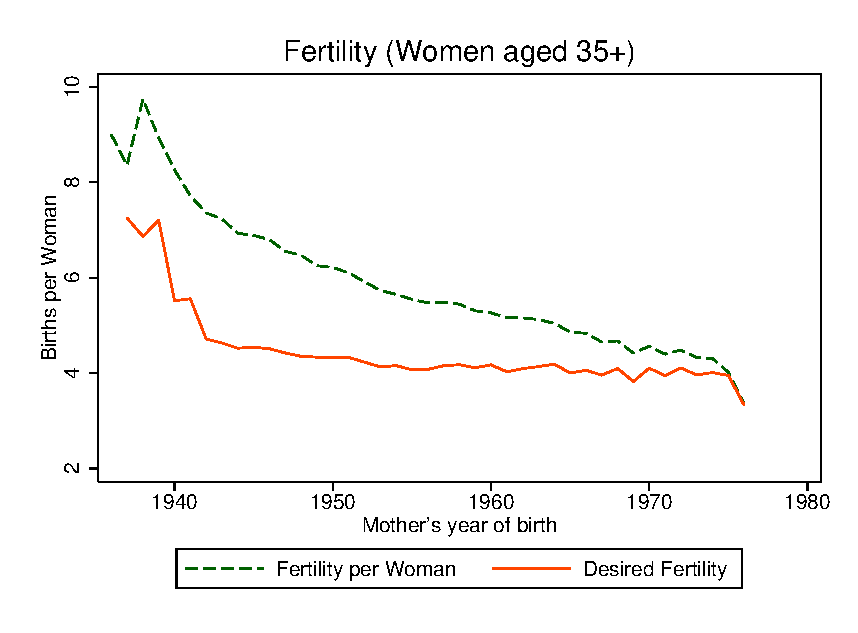
\includegraphics[scale=0.53]{\twinfolder/Figures/ferttrend_35_all.eps}
  \caption{Trends in Fertility}
  \label{TWINfig:fertrend}
\end{subfigure}%
\begin{subfigure}{.5\textwidth}
  \centering
  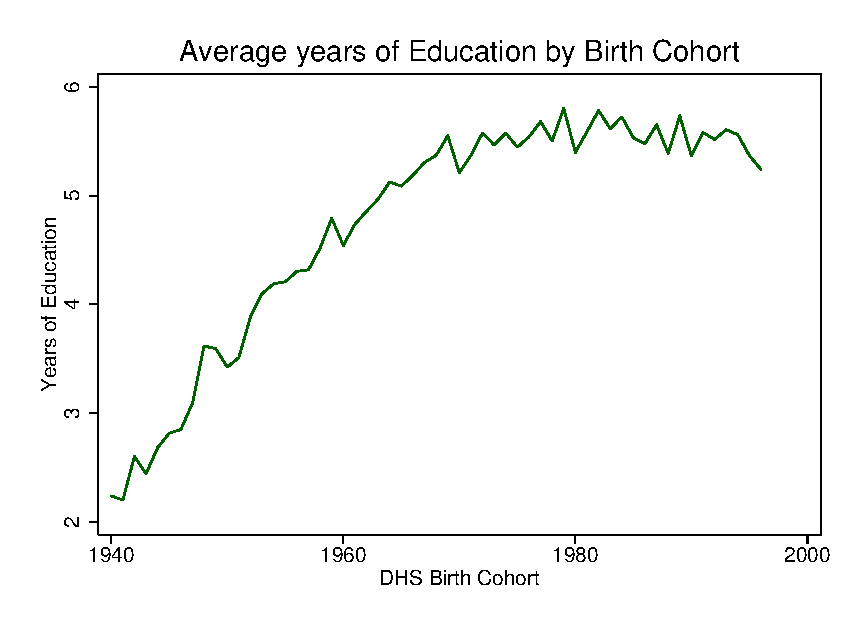
\includegraphics[scale=0.52]{\twinfolder/Figures/eductrend_all.eps}
  \caption{Trend in Education}
  \label{TWINfig:eductrend}
\end{subfigure}
\caption{Education and Fertility}
\label{TWINfig:trends}
\floatfoot{Note to figure \ref{TWINfig:trends}: Cohorts are made up of all individuals 
from the DHS who are over 35 years (for fertility), and over 15 years (for education).  
In each case the sample is restricted to those who have approximately completed fertility 
and education respectively.}
\end{figure}
\vspace{1cm}

\begin{figure}[htpb!]
\begin{center}
\caption{Proportion of Twins by Birth Order}
\label{TWINfig:bord}
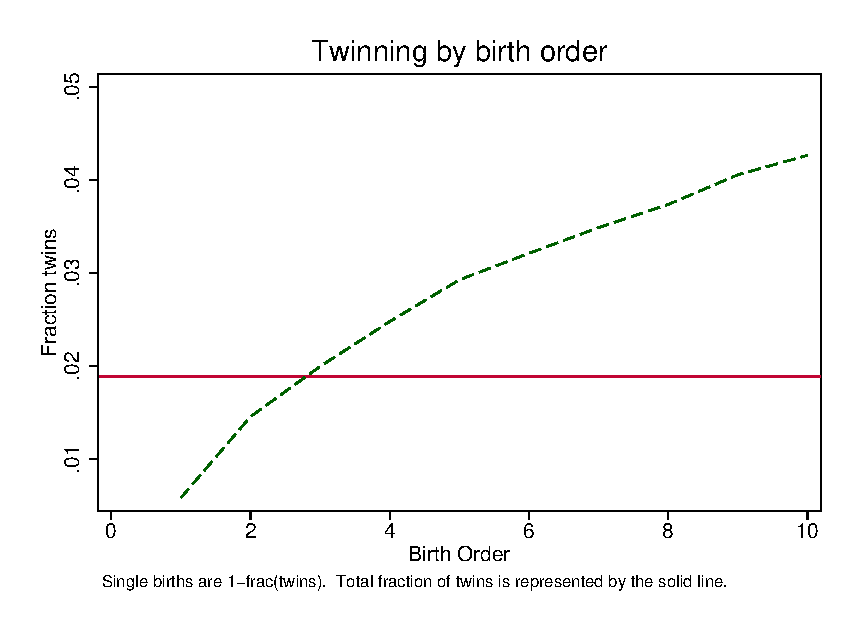
\includegraphics[scale=0.92]{\twinfolder/Figures/twinbybord.eps} 
\end{center}
\end{figure}

\begin{figure}[htpb!]
\begin{center}
\caption{Twin Births and Total Fertility}
\label{TWINfig:births}
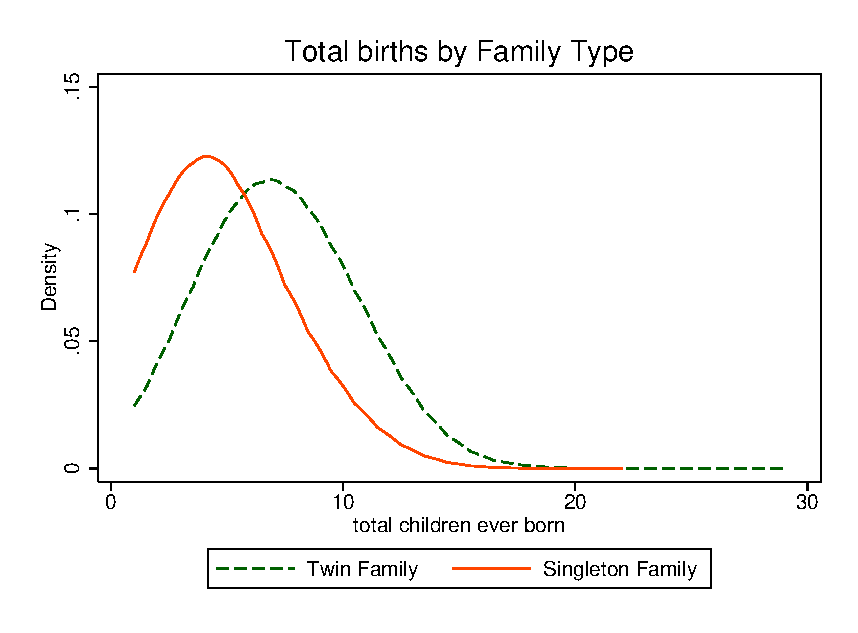
\includegraphics[scale=0.92]{\twinfolder/Figures/famsize.eps} 
\end{center}
\end{figure}

\begin{figure}[htpb!]
\begin{center}
\caption{Intra- and Inter-country trends: height and twinning}
\label{TWINfig:arrows}
\includegraphics[scale=0.86]{\twinfolder/Figures/height_country.eps} 
\end{center}
\end{figure}

\begin{figure}[htpb!]
\begin{center}
\caption{Proportion of Twins of All Births (USA)}
\label{TWINfig:USTwin}
\includegraphics[scale=0.92]{\twinfolder/Figures/USTwinFLE.eps} 
\end{center}
\end{figure}

\begin{figure}[htpb!]
\begin{center}
\caption{Relaxing Strict Exogeneity (two plus)}
\label{TWINfig:ltz2}
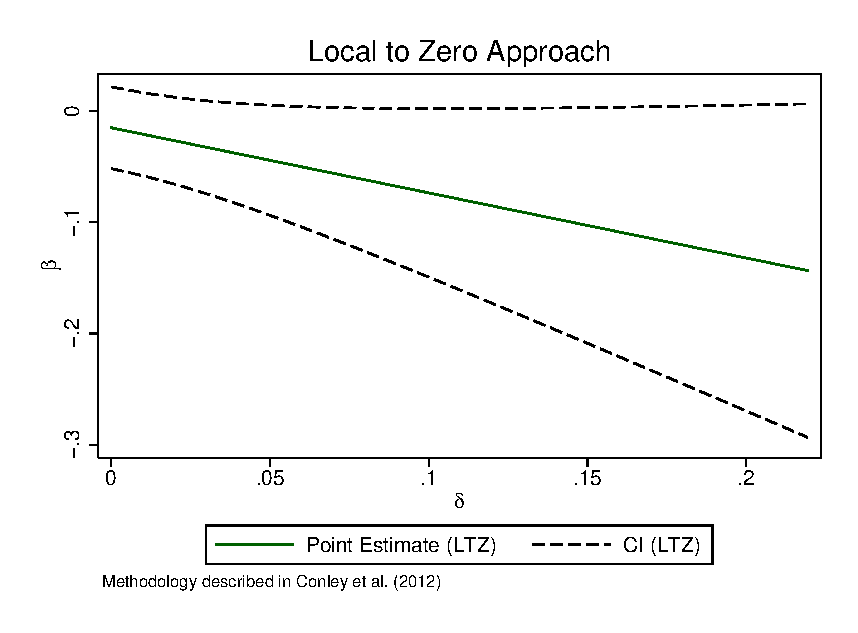
\includegraphics[scale=0.88]{\twinfolder/Figures/LTZ_two.eps}
\vspace{-8mm}
\floatfoot{Note to figure \ref{TWINfig:ltz2}: See note to Figure \ref{TWINfig:ltz3}}
\end{center}
\end{figure}

\begin{figure}[htpb!]
\begin{center}
\caption{Relaxing Strict Exogeneity (three plus)}
\label{TWINfig:ltz3}
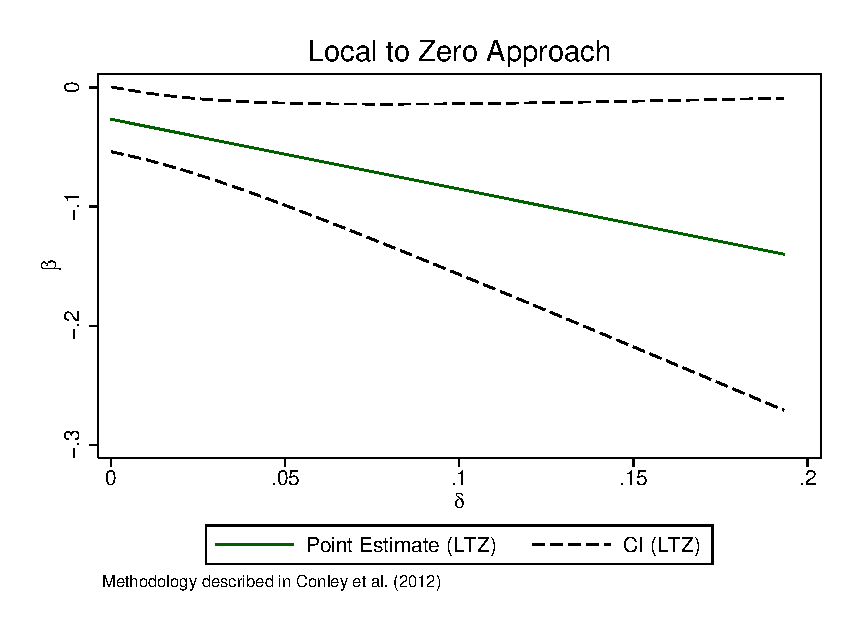
\includegraphics[scale=0.88]{\twinfolder/Figures/LTZ_three.eps} 
\floatfoot{Note to figure \ref{TWINfig:ltz3}: Confidence intervals and point estimates 
are calculated according to \citet{Conleyetal2012}.  Estimates reflect a range of priors 
regarding the validity of the exclusion restriction required to consistently estimate 
$\hat\beta_{fert}$ using twinning in a 2SLS framework.  The local to zero (LTZ) 
approach applied here assumes that $\gamma$, the sign on the instrument when included
in the first stage, is distributed $\gamma\sim U(0,\delta)$.  Further discussion 
is provided in the body of the text and table \ref{TWINtab:Conley}.}
\end{center}
\end{figure}




\section*{Tables}
Begin overleaf.

\begin{landscape}\begin{table}[htpb!] 
\caption{Probability of Giving Birth to Twins} \label{TWINtab:twinreg1} 
\begin{center}\begin{tabular}{lcccccc} \toprule \toprule 
&(1)&(2)&(3)&(4)&(5)&(6)\\
Twin*100&All&\multicolumn{2}{c}{Income}&\multicolumn{2}{c}{Time}&Prenatal\\
 \cmidrule(r){3-4} \cmidrule(r){5-6} 
&&Low inc&Middle inc&1990-2013&1972-1989&\\\midrule
\begin{footnotesize}\end{footnotesize}&\begin{footnotesize}\end{footnotesize}&\begin{footnotesize}\end{footnotesize}&\begin{footnotesize}\end{footnotesize}&\begin{footnotesize}\end{footnotesize}&\begin{footnotesize}\end{footnotesize}&\begin{footnotesize}\end{footnotesize}\\
Age&0.596***&0.615***&0.554***&0.647***&0.326***&0.631***\\
&(0.029)&(0.036)&(0.050)&(0.033)&(0.075)&(0.040)\\
Age Squared&-0.008***&-0.008***&-0.008***&-0.009***&-0.003**&-0.009***\\
&(0.001)&(0.001)&(0.001)&(0.001)&(0.001)&(0.001)\\
Age First Birth&-0.053***&-0.093***&0.004&-0.052***&-0.056***&-0.041***\\
&(0.009)&(0.012)&(0.014)&(0.010)&(0.019)&(0.013)\\
Education (years)&0.042**&0.089***&-0.005&0.048**&0.022&-0.068**\\
&(0.017)&(0.022)&(0.029)&(0.020)&(0.034)&(0.028)\\
Education squared&-0.002&-0.006***&0.001&-0.002&0.000&0.003\\
&(0.001)&(0.002)&(0.002)&(0.002)&(0.003)&(0.002)\\
Height&0.058***&0.057***&0.059***&0.062***&0.042***&0.058***\\
&(0.004)&(0.005)&(0.007)&(0.005)&(0.008)&(0.007)\\
BMI&0.048***&0.063***&0.039***&0.046***&0.055***&0.044***\\
&(0.006)&(0.009)&(0.009)&(0.007)&(0.011)&(0.011)\\
Prenatal (Doctor)&&&&&&0.906***\\
&&&&&&(0.128)\\
Prenatal (Nurse)&&&&&&0.067\\
&&&&&&(0.108)\\
Prenatal (None)&&&&&&-0.497***\\
&&&&&&(0.132)\\
&&&&&&\\R-squared&0.01&0.01&0.01&0.01&0.01&0.01\\
Observations &1930653&1201555&729098&1524947&405706&615935\\
\hline\hline\multicolumn{7}{p{14.3cm}}{\begin{footnotesize}\textsc{Notes:} All specifications include a full set of year of birth and  country dummies, and are estimated as linear probability models.  Twin is multiplied by 100 for presentation.  Height is measured in cm  and BMI is weight in kg divided by height in metres squared. l  Prenatal care variables are only recoreded for recent births.  As  such, column (6) is estimated only for that subset of births where  these observations are made.
$^{*}$p$<$0.1; $^{**}$p$<$0.05; $^{***}$p$<$0.01
 \end{footnotesize}}\\ \hline \normalsize \end{tabular}\end{center}\end{table}\end{landscape} 

\begin{table}[htpb!]
\caption{United States Birth Registry (Administrative 2003-2012)}
\begin{center}
\scalebox{0.54}{
\begin{tabular}{lcccc} \hline
 & (1) & (2) & (3) & (4) \\
VARIABLES & twin100 & twin100 & twin100 & twin100 \\ \hline
\vspace{4pt} & \begin{footnotesize}\end{footnotesize} & \begin{footnotesize}\end{footnotesize} & \begin{footnotesize}\end{footnotesize} & \begin{footnotesize}\end{footnotesize} \\
africanAmerican & 0.554*** & 0.437*** & 0.437*** & 0.331*** \\
\vspace{4pt} & \begin{footnotesize}(0.00911)\end{footnotesize} & \begin{footnotesize}(0.0142)\end{footnotesize} & \begin{footnotesize}(0.0142)\end{footnotesize} & \begin{footnotesize}(0.0143)\end{footnotesize} \\
otherRace & 0.0433*** & 0.135*** & 0.135*** & -0.680*** \\
\vspace{4pt} & \begin{footnotesize}(0.00886)\end{footnotesize} & \begin{footnotesize}(0.0148)\end{footnotesize} & \begin{footnotesize}(0.0148)\end{footnotesize} & \begin{footnotesize}(0.0200)\end{footnotesize} \\
meducSecondary & 0.00124 & 0.0124 & 0.0124 & 0.810*** \\
\vspace{4pt} & \begin{footnotesize}(0.00881)\end{footnotesize} & \begin{footnotesize}(0.0159)\end{footnotesize} & \begin{footnotesize}(0.0159)\end{footnotesize} & \begin{footnotesize}(0.0203)\end{footnotesize} \\
meducTertiary & 1.124*** & 1.110*** & 1.110*** & 2.063*** \\
\vspace{4pt} & \begin{footnotesize}(0.00930)\end{footnotesize} & \begin{footnotesize}(0.0158)\end{footnotesize} & \begin{footnotesize}(0.0158)\end{footnotesize} & \begin{footnotesize}(0.0209)\end{footnotesize} \\
tobaccoUse & -0.327*** & -0.424*** & -0.424*** & -0.422*** \\
\vspace{4pt} & \begin{footnotesize}(0.0126)\end{footnotesize} & \begin{footnotesize}(0.0181)\end{footnotesize} & \begin{footnotesize}(0.0181)\end{footnotesize} & \begin{footnotesize}(0.0182)\end{footnotesize} \\
alcoholUse &  & -1.233*** & -1.233*** & -1.182*** \\
\vspace{4pt} & \begin{footnotesize}\end{footnotesize} & \begin{footnotesize}(0.0648)\end{footnotesize} & \begin{footnotesize}(0.0648)\end{footnotesize} & \begin{footnotesize}(0.0651)\end{footnotesize} \\
anemia &  &  &  & -1.349*** \\
\vspace{4pt} & \begin{footnotesize}\end{footnotesize} & \begin{footnotesize}\end{footnotesize} & \begin{footnotesize}\end{footnotesize} & \begin{footnotesize}(0.0335)\end{footnotesize} \\
diabetes &  &  &  & -0.408*** \\
\vspace{4pt} & \begin{footnotesize}\end{footnotesize} & \begin{footnotesize}\end{footnotesize} & \begin{footnotesize}\end{footnotesize} & \begin{footnotesize}(0.0280)\end{footnotesize} \\
chyper &  &  &  & -0.883*** \\
\vspace{4pt} & \begin{footnotesize}\end{footnotesize} & \begin{footnotesize}\end{footnotesize} & \begin{footnotesize}\end{footnotesize} & \begin{footnotesize}(0.0528)\end{footnotesize} \\
phyper &  &  &  & -4.128*** \\
\vspace{4pt} & \begin{footnotesize}\end{footnotesize} & \begin{footnotesize}\end{footnotesize} & \begin{footnotesize}\end{footnotesize} & \begin{footnotesize}(0.0267)\end{footnotesize} \\
eclamp &  &  &  & -5.686*** \\
\vspace{4pt} & \begin{footnotesize}\end{footnotesize} & \begin{footnotesize}\end{footnotesize} & \begin{footnotesize}\end{footnotesize} & \begin{footnotesize}(0.0896)\end{footnotesize} \\
Constant & 5.461*** & 5.326*** & 5.326*** & 32.75*** \\
 & \begin{footnotesize}(0.0525)\end{footnotesize} & \begin{footnotesize}(0.0806)\end{footnotesize} & \begin{footnotesize}(0.0806)\end{footnotesize} & \begin{footnotesize}(0.293)\end{footnotesize} \\
\vspace{4pt} & \begin{footnotesize}\end{footnotesize} & \begin{footnotesize}\end{footnotesize} & \begin{footnotesize}\end{footnotesize} & \begin{footnotesize}\end{footnotesize} \\
Observations & 38,910,055 & 16,605,619 & 16,605,619 & 12,219,256 \\
 $R^2$ & 0.008 & 0.008 & 0.008 & 0.012 \\ \hline
\multicolumn{5}{c}{\begin{footnotesize} Standard errors in parentheses\end{footnotesize}} \\
\multicolumn{5}{c}{\begin{footnotesize} *** p$<$0.01, ** p$<$0.05, * p$<$0.1\end{footnotesize}} \\
\end{tabular}}
\end{center}
\end{table}

\input{\twinfolder/Tables/TwinRegs/ChileTwin.tex}
\input{\twinfolder/Tables/TwinRegs/ScotlandTwin.tex}
\input{\twinfolder/Tables/TwinRegs/SwedenTwin2.tex}
\input{\twinfolder/Tables/Stress.tex}
\begin{table}[htpb]
\caption{Probability of Giving Births to Twins (NHIS, USA)}
\begin{center}
\scalebox{0.64}{
\begin{tabular}{lcc} \toprule
&(1)&(2) \\
VARIABLES&Twin$\times$100&Twin$\times$100 \\ \midrule
&& \\
Mother's Height&0.0416**&0.0406** \\
&(0.0201)&(0.0201) \\
Mother's Education&0.0084&0.0033 \\
&(0.0162)&(0.0164) \\
Smokes (pre-Pregnancy)&-0.119&-0.0983 \\
&(0.115)&(0.116) \\
Mother's Age&0.0121&0.0108 \\
&(0.0446)&(0.0446) \\
Mother's Age$^2$ &-0.0008&-0.0008 \\
&(0.0006)&(0.0006) \\
Age First Birth &0.166***&0.164*** \\
&(0.0135)&(0.0136) \\
BMI &0.0123***&0.0130*** \\
&(0.0034)&(0.0034) \\
Mother Good Health&&0.203* \\
&&(0.116) \\
Mother Poor Health&&-0.00284 \\
&&(0.189) \\
Constant&-4.091***&-4.101*** \\
&(1.542)&(1.543) \\
&& \\
Observations&105,879&105,879 \\
R-squared&0.004&0.004 \\ \midrule
%\multicolumn{3}{ p{5cm} }{\begin{footnotesize}\textsc{Notes:} Standard errors in parentheses. *** p$<$0.01; ** p$<$0.05; * p$<$0.1\end{footnotesize}}\bottomrule
\end{tabular}}
\end{center}
\end{table}

\input{\twinfolder/Tables/USfdeaths.tex}
\begin{table}
\caption{Twins, Miscarriage and Maternal Health (Administrative Data from Spain)}
\begin{center}
\scalebox{0.76}{
\begin{tabular}{lclc}
\hline 
VARIABLES	&	Fetal Death$	\times$100 & & \\	\hline
	&	(1) & &	\\
Primary	&	  -0.60179*** &	Primary$	\times$Twin	&	   -0.6618***	\\
	&	 (0.01456)	& &	 (0.20926)	\\
Secondary	&	  -0.71998*	& Secondary$	\times$Twin	&	  -0.55901***	\\
	&	  (0.0151)	& 	&	 .0020978	\\
Tertiary	&	  -0.80019***	& Tertiary$	\times$Twin	&	  -0.65091***	\\
	&	(0.01582)	& 	&	(0.20866)	\\
Immigration	&	  -0.07223***	& Immigration$	\times$Twin	&	  0.22871	\\
	&	 (0.0171)	& 	&	(0.29614)	\\
City	&	  -0.00321	& City$	\times$Twin	&	  0.09566	\\
	&	(0.01584)	& 	&	 (0.26876)	\\
Married	&	  -0.07354***	&Married$	\times$Twin	&	  -0.08978	\\
	&	 (0.00759)	&	&	 (0.11893)	\\
No Father	&	0.68626***	&No Father$	\times$Twin	&	3.25232	\\
	&	 (0.23825)	&	&	(4.09309)	\\
Constant	&	-1.35966***	& & \\
	&	(0.33674)	& &  \\
	& \\
	Obs & 2,869,329 & & \\
	$R^2$ & 0.0044  & & \\ \midrule
	\multicolumn{4}{p{8cm}}{Note: Spanish administrative births: 2007-2012.}
\end{tabular}}
\end{center}
\end{table}



\clearpage


\bibliography{./BiBBase1}

\newpage
%*******************************************************************************
\appendix
\section*{Appendices}
\section{Data Appendix}
\label{TWINscn:dataApp}
Main IV and OLS results for this paper are based on DHS and NHIS data described 
in section \ref{TWINscn:data}.  These data are downloaded directly off the web 
and merged to form the estimation samples of interest. For DHS data, we use two 
surveys: the Individual (woman) Recode (IR), and the Household Recode (HR) 
providing education for each household member.  For NHIS data, we merge three 
of the datafiles made available by the CDC: familyxx, household, and person.
In each case, full generating code for this process is made available on the
authors' websites.  This code downloads, merges and cleans DHS and NHIS data to
produce the datasets (one line per child) used in analysis.

In auxiliary regressions examining the characterstics of mothers and the 
relationship these characteristics and twin births and miscarriage, we consult
a large number of other datasets.  These are the following:
\begin{itemize}
\item United States National Vital Statistics Birth Data
\item United States National Vital Statistics Fetal Death Data
\item Spanish Vital Statistics (INE)
\item The Swedish Medical Birth Register
\item Scottish Vital Statistics
\item Longitudinal Early Life Survey, Chile (ELPI) 
\end{itemize}

In the case of the first 5 datasets (administrative records of births and/or 
fetal deaths), we use all recorded instances, focusing on twins as our 
outcome variable of interest.  Depending upon the data source, we use all
available measures of pre-determined maternal health stocks or family 
socioeconomic indicators.  The ELPI survey from Chile focuses on child early
life, and records mother's behaviours before, during and after pregnancy,
along with child birth outcomes.  We use all children from the first wave of
this survey to run the twin regression included in the appendix tables.  
Further notes regarding each dataset and the particular years and number of
births can be found in the notes to each table.

\section{Plausibly Exogenous Bounds and Estimating $\gamma$}
\label{TWINscn:gamma}
From (\ref{TWINeqn:Conley}), we are interested in forming a consistent estimate
of $\gamma=\frac{\partial educ}{\partial twin}\big|_{X}$. From 
\citet{BhalotraVenkataramani2014} we have:
\begin{equation}
\label{TWINeqn:BV}
Y_{stc} = \alpha + \phi (Post_t\times basePneumonia_s) +\theta_{rs} +\eta_{rt}
+\varphi\mathbf{X}_{st}+\lambda_{rc}+\theta_s\times\eta_t+\varepsilon_{stc}
\end{equation}
where $\phi$ is the effect of access to sulfanide drugs on the outcome variable 
$Y_{stc}$.\footnote{This is an unbiased effect of sulfanide drugs on health if
parallel trends are satisfied between high- and low-intensity states. Evidence of
this is provided by \citet{BhalotraVenkataramani2014}.}
Let's consider estimating the effect of this exogenous shock to maternal health
on child quality:
\begin{equation}
\label{TWINeqn:BV1}
%\begin{subequations}
%\begin{eqnarray}
%\label{TWINeqn:BV1}
%Pr(Twin)_{stc} &=& \alpha^t + \phi^t (Post_t\times basePneumonia_s) +\cdots +\varepsilon^t_{stc} \\
%\label{TWINeqn:BV2}
educ_{stc} = \alpha^q + \phi^q (Post_t\times basePneumonia_s) +\cdots+\varepsilon^q_{stc} 
%\end{eqnarray}
%\end{subequations}
\end{equation}
%*******************************************************************************
where superscript $q$ refers to coefficients in the quality regression, and the 
remainder of (\ref{TWINeqn:BV1}) follows specification (\ref{TWINeqn:BV}).  
Under typical difference-in-difference assumptions, we can thus causally 
estimate $\phi^q=\frac{\partial educ}{\partial bP}\big|_{X}$ by OLS (where $bP$ 
is the $Post_t\times basePneumonia_s$ variable).  

From (\ref{TWINeqn:BV1}) we isolate the effect of a positive maternal health 
shock (the reduction in rates of pneumonia) on child quality.  However, for 
$\gamma$---the violation of the exclusion restriction---we need to estimate the 
twin-mediated effect of health shocks on child quality.  Thus, to estimate 
$\gamma$, we must know both the effect of a particular health shock on quality
($\phi^q$), as well as the relative levels of health of twin and non-twin 
mothers.\footnote{As a simple example, if the effect of a maternal health 
variable is to increase child quality by 0.1 standard deviations, and twin 
mothers have 20\% higher stocks of that maternal health variable than non-twin 
mothers, this suggests an estimate of $\gamma$ (the twin-mediated effect of
maternal health on child quality) of 0.1*0.2=0.02 s.d.}  We refer to this as
quantity as $\phi^t$, and this captures the difference in average rates of 
(state) pneumonia mortality between twin and non-twin families:
\begin{equation}
\label{TWINeqn:BV2}
\phi^t=\overline{bP}_{twin=1}-\overline{bP}_{twin=0}=
\frac{\partial bP}{\partial twin}\bigg|_{X},
%$\phi^t=\frac{\partial twin}{\partial bP}\big|_{X}$ and
\end{equation}
where we condition on the controls from (\ref{TWINeqn:BV1}).  Finally, with 
these two quantities in hand, we can estimate $\gamma$ by taking their product:
\begin{equation}
\label{TWINeqn:realgamma}
\phi^q\times\phi^t=\frac{\partial educ}{\partial bP}\times
\frac{\partial bP}{\partial twin}\bigg|_{X}=
\frac{\partial educ}{\partial twin}\bigg|_{X}=\gamma.
\end{equation}
This is our estimand of interest, and we can plug it into our estimates of
the bounds on $\beta_1$ using \citeauthor{Conleyetal2012}'s method.

%*******************************************************************************
In order to estimate (\ref{TWINeqn:realgamma}) we turn to US census data 
described in \citet{BhalotraVenkataramani2014}, firstly estimate $\phi^t$ and 
$\phi^q$, and then calculate ratio of these values to form an estimate of 
$\gamma$, which we denote $\hat\gamma$.  In the case of the UCI approach, this 
is sufficient to estimate the bounds of $\beta_1$, assuming that: 
$\gamma\in[0,2\hat\gamma]$.\footnote{We scale $\hat\gamma$ by the factor of 2 in 
order for this value to fall precisely in the middle of the range. 
\citet{Conleyetal2012} provide a similar example to calculate the returns to 
education using the UCI approach.} In the case of the more precise LTZ approach 
(our preferred bounds estimates), the logic is similar, however now we must form 
a prior over the entire distribution of $\gamma$.  Calculating the variance of 
$\gamma$ is not as straightforward as using the variance-covariance matrix 
corresponding to each of the estimates $\hat\phi^t$ and $\hat\phi^q$.  In this 
case however we can use bootstrapping to calculate $J$ replications of 
$\hat\phi^t\times\hat\phi^q$, and from these estimates construct an estimated 
distribution of $\hat\gamma$, which allows us to determine our prior for the 
distribution of $\gamma$.  From this empirical distribution, we observe the 
estimated mean and standard deviation, and finally test whether the distribution 
is normal using a Shapiro Wilk test for normality.\footnote{We also use 
Kolmogorov-Smirnov tests for equality of distributions to test whether the 
distribution is more likely to be log normal, uniform, and a number of other
analytical distributions. In order to do this, we first estimate the empirical 
distribution as described previously.  We then observe the mean $\hat\mu$ and 
the standard deviation $\hat\sigma$, and run a one-sample test do determine 
whether the observed empirical distribution is is significantly different to 
each analytical distribution $\mathcal{N}(\hat\mu,\hat\sigma^2)$, 
$U(\hat\mu,\hat\sigma^2)$ or $\ln\mathcal{N}(\hat\mu,\hat\sigma^2)$.}

\newpage
\end{spacing}

\section{Appendix Tables}
\setcounter{table}{0}
\renewcommand{\thetable}{A\arabic{table}}

\begin{table}[htpb!]
\caption{United States Birth Registry (Administrative 2003-2012)}
\begin{center}
\scalebox{0.54}{
\begin{tabular}{lcccc} \hline
 & (1) & (2) & (3) & (4) \\
VARIABLES & twin100 & twin100 & twin100 & twin100 \\ \hline
\vspace{4pt} & \begin{footnotesize}\end{footnotesize} & \begin{footnotesize}\end{footnotesize} & \begin{footnotesize}\end{footnotesize} & \begin{footnotesize}\end{footnotesize} \\
africanAmerican & 0.554*** & 0.437*** & 0.437*** & 0.331*** \\
\vspace{4pt} & \begin{footnotesize}(0.00911)\end{footnotesize} & \begin{footnotesize}(0.0142)\end{footnotesize} & \begin{footnotesize}(0.0142)\end{footnotesize} & \begin{footnotesize}(0.0143)\end{footnotesize} \\
otherRace & 0.0433*** & 0.135*** & 0.135*** & -0.680*** \\
\vspace{4pt} & \begin{footnotesize}(0.00886)\end{footnotesize} & \begin{footnotesize}(0.0148)\end{footnotesize} & \begin{footnotesize}(0.0148)\end{footnotesize} & \begin{footnotesize}(0.0200)\end{footnotesize} \\
meducSecondary & 0.00124 & 0.0124 & 0.0124 & 0.810*** \\
\vspace{4pt} & \begin{footnotesize}(0.00881)\end{footnotesize} & \begin{footnotesize}(0.0159)\end{footnotesize} & \begin{footnotesize}(0.0159)\end{footnotesize} & \begin{footnotesize}(0.0203)\end{footnotesize} \\
meducTertiary & 1.124*** & 1.110*** & 1.110*** & 2.063*** \\
\vspace{4pt} & \begin{footnotesize}(0.00930)\end{footnotesize} & \begin{footnotesize}(0.0158)\end{footnotesize} & \begin{footnotesize}(0.0158)\end{footnotesize} & \begin{footnotesize}(0.0209)\end{footnotesize} \\
tobaccoUse & -0.327*** & -0.424*** & -0.424*** & -0.422*** \\
\vspace{4pt} & \begin{footnotesize}(0.0126)\end{footnotesize} & \begin{footnotesize}(0.0181)\end{footnotesize} & \begin{footnotesize}(0.0181)\end{footnotesize} & \begin{footnotesize}(0.0182)\end{footnotesize} \\
alcoholUse &  & -1.233*** & -1.233*** & -1.182*** \\
\vspace{4pt} & \begin{footnotesize}\end{footnotesize} & \begin{footnotesize}(0.0648)\end{footnotesize} & \begin{footnotesize}(0.0648)\end{footnotesize} & \begin{footnotesize}(0.0651)\end{footnotesize} \\
anemia &  &  &  & -1.349*** \\
\vspace{4pt} & \begin{footnotesize}\end{footnotesize} & \begin{footnotesize}\end{footnotesize} & \begin{footnotesize}\end{footnotesize} & \begin{footnotesize}(0.0335)\end{footnotesize} \\
diabetes &  &  &  & -0.408*** \\
\vspace{4pt} & \begin{footnotesize}\end{footnotesize} & \begin{footnotesize}\end{footnotesize} & \begin{footnotesize}\end{footnotesize} & \begin{footnotesize}(0.0280)\end{footnotesize} \\
chyper &  &  &  & -0.883*** \\
\vspace{4pt} & \begin{footnotesize}\end{footnotesize} & \begin{footnotesize}\end{footnotesize} & \begin{footnotesize}\end{footnotesize} & \begin{footnotesize}(0.0528)\end{footnotesize} \\
phyper &  &  &  & -4.128*** \\
\vspace{4pt} & \begin{footnotesize}\end{footnotesize} & \begin{footnotesize}\end{footnotesize} & \begin{footnotesize}\end{footnotesize} & \begin{footnotesize}(0.0267)\end{footnotesize} \\
eclamp &  &  &  & -5.686*** \\
\vspace{4pt} & \begin{footnotesize}\end{footnotesize} & \begin{footnotesize}\end{footnotesize} & \begin{footnotesize}\end{footnotesize} & \begin{footnotesize}(0.0896)\end{footnotesize} \\
Constant & 5.461*** & 5.326*** & 5.326*** & 32.75*** \\
 & \begin{footnotesize}(0.0525)\end{footnotesize} & \begin{footnotesize}(0.0806)\end{footnotesize} & \begin{footnotesize}(0.0806)\end{footnotesize} & \begin{footnotesize}(0.293)\end{footnotesize} \\
\vspace{4pt} & \begin{footnotesize}\end{footnotesize} & \begin{footnotesize}\end{footnotesize} & \begin{footnotesize}\end{footnotesize} & \begin{footnotesize}\end{footnotesize} \\
Observations & 38,910,055 & 16,605,619 & 16,605,619 & 12,219,256 \\
 $R^2$ & 0.008 & 0.008 & 0.008 & 0.012 \\ \hline
\multicolumn{5}{c}{\begin{footnotesize} Standard errors in parentheses\end{footnotesize}} \\
\multicolumn{5}{c}{\begin{footnotesize} *** p$<$0.01, ** p$<$0.05, * p$<$0.1\end{footnotesize}} \\
\end{tabular}}
\end{center}
\end{table}

\input{\twinfolder/Tables/TwinRegs/ChileTwin.tex}
\input{\twinfolder/Tables/TwinRegs/USfdeaths.tex}
\begin{table}
\caption{Twins, Miscarriage and Maternal Health (Administrative Data from Spain)}
\begin{center}
\scalebox{0.76}{
\begin{tabular}{lclc}
\hline 
VARIABLES	&	Fetal Death$	\times$100 & & \\	\hline
	&	(1) & &	\\
Primary	&	  -0.60179*** &	Primary$	\times$Twin	&	   -0.6618***	\\
	&	 (0.01456)	& &	 (0.20926)	\\
Secondary	&	  -0.71998*	& Secondary$	\times$Twin	&	  -0.55901***	\\
	&	  (0.0151)	& 	&	 .0020978	\\
Tertiary	&	  -0.80019***	& Tertiary$	\times$Twin	&	  -0.65091***	\\
	&	(0.01582)	& 	&	(0.20866)	\\
Immigration	&	  -0.07223***	& Immigration$	\times$Twin	&	  0.22871	\\
	&	 (0.0171)	& 	&	(0.29614)	\\
City	&	  -0.00321	& City$	\times$Twin	&	  0.09566	\\
	&	(0.01584)	& 	&	 (0.26876)	\\
Married	&	  -0.07354***	&Married$	\times$Twin	&	  -0.08978	\\
	&	 (0.00759)	&	&	 (0.11893)	\\
No Father	&	0.68626***	&No Father$	\times$Twin	&	3.25232	\\
	&	 (0.23825)	&	&	(4.09309)	\\
Constant	&	-1.35966***	& & \\
	&	(0.33674)	& &  \\
	& \\
	Obs & 2,869,329 & & \\
	$R^2$ & 0.0044  & & \\ \midrule
	\multicolumn{4}{p{8cm}}{Note: Spanish administrative births: 2007-2012.}
\end{tabular}}
\end{center}
\end{table}


\clearpage
\newpage

\section{Appendix Figures}
\setcounter{figure}{0}
\renewcommand{\thefigure}{A\arabic{figure}}

\begin{figure}[htpb!]
\begin{center}
\caption{Birth Size of Twins versus Singeltons}
\label{TWINfig:Size}
\includegraphics[scale=0.90]{\twinfolder/Figures/Size.eps} 
\end{center}
\end{figure}

\begin{figure}[htpb!]
\begin{center}
\caption{Height and Selective Survival}
\label{TWINfig:survival}
\includegraphics[scale=0.90]{\twinfolder/Figures/MMRcuts.eps} 
\end{center}
\end{figure}

\begin{figure}[htpb!]
\begin{center}
\caption{Bootstrap Estimates of $\hat\gamma$}
\label{TWINfig:gammaBoots}
\includegraphics[scale=0.90]{\twinfolder/Figures/gammaResamp.eps} 
\end{center}
\floatfoot{Note to figure \ref{TWINfig:gammaBoots}: The empirical distribution
is generated by performing J=100 bootstrap replications to estimate $\phi_t$ and
$\phi_q$ (see discussion in appendix \ref{TWINscn:gamma}).  The analytical 
distribution is a normal $\sim N(\mu_{\hat\gamma},\sigma_{\hat\gamma})$.  The
values estimated in the bootstrap replications are $\mu_{\hat\gamma}=0.0642$ and
$\sigma_{\hat\gamma}=0.0493$.}
\end{figure}


\appendix
\section*{Online Appendices}
\section{Tables}
\setcounter{table}{0}
\renewcommand{\thetable}{B\arabic{table}} 

\input{\twinfolder/Tables/Countries.tex}
\input{\twinfolder/Tables/Balance_mother2_3.tex}



\end{document}


%%********************************************************************************
Estimation of the Q-Q model using twin births to instrument fertility relies on 
the fact that twin births are exogenous. This implies that both conceiving twins 
\emph{and} taking them to term cannot depend on maternal behaviours and health 
stocks. In this paper we suggest that such an assumption may be too strong to 
hold in practice. We show that healthier mothers are more likely to give birth to 
twins even if twin conception is random, and that the size of this effect is 
considerable.

We re-estimate the Q-Q tradeoff accounting for such an effect.  We thus show
that the existing wisdom (which suggests that the effect of additional births 
on human capital might be minor), likely underestimates the true magnitude of
the Q-Q tradeoff.  Our IV estimates move point estimates from approximately 
0\% of a standard deviation (using the old methodology which does not account
for maternal health) to a significant $-4\%$ of a standard deviation of 
educational attainment.  Further, we suggest that this is likely
a lower bound of the true effect.  Depending upon the degree to which maternal
characteristics predict twin births, the true trade-off may be considerably
larger, perhaps even doubling these IV estimates.  The availability of richer 
maternal health and behaviour data in surveys would allow for us to restrict
the size of these bounds and produce more precise estimates.


